\documentclass[11pt,a4paper]{report}

%https://tex.stackexchange.com/questions/134079/font-setup-for-an-academic-thesis-no-computer-modern-wanted
%\usepackage[libertine,cmintegrals,cmbraces,vvarbb]{newtxmath}
%\usepackage[scaled=0.95]{inconsolata}
%\usepackage{classicthesis}

\usepackage[sc]{mathpazo}

%\usepackage{helvet}
%\renewcommand{\familydefault}{\sfdefault}

%\usepackage{lmodern}

\linespread{1.2}
\usepackage[margin=1in]{geometry}

\usepackage{microtype}
\usepackage{wrapfig}

\usepackage[sort,numbers,sectionbib]{natbib}
%\usepackage{natbib}
%\usepackage{biblatex}
\bibliographystyle{IEEEtranUrldate}
\renewcommand{\bibname}{References}
%\usepackage{urlbst}

% http://ctan.org/pkg/lipsum
\usepackage{lipsum}

% https://tex.stackexchange.com/questions/94224/how-to-create-a-list-with-a-fixed-prefix-and-incremental-numbers
\usepackage{enumitem}

% strikethrough st
\usepackage{soul}

% https://tex.stackexchange.com/questions/86120/font-size-of-figure-caption-header
\usepackage[font=scriptsize,labelfont=bf]{caption}

%https://tex.stackexchange.com/questions/3001/list-sections-of-chapter-at-beginning-of-that-chapter
% !!! NEEDS TO BE ABOVE HYPEREF !!!
\usepackage{titletoc}

% https://www.sharelatex.com/learn/Hyperlinks
\usepackage{hyperref}
\hypersetup{
    colorlinks,
    %citecolor=gray,
    citecolor=blue,
    filecolor=black,
    linkcolor=blue,
    urlcolor=blue,
    linktoc=all
}

\usepackage[nameinlink,capitalise,noabbrev]{cleveref}

% includegraphics
\usepackage[]{graphicx}
\graphicspath{{../img/}}
\usepackage{mwe}

\usepackage[outputdir=build]{minted}
%https://www.sharelatex.com/learn/Code_Highlighting_with_minted#Reference_guide
%\usemintedstyle{vs}
% https://tex.stackexchange.com/questions/161124/how-to-make-a-minted-code-listing-centered-on-a-page
% WARNING MAKES LONG CODE on 1 page!
%\RecustomVerbatimEnvironment{Verbatim}{BVerbatim}{}
\setminted[verilog]{linenos,baselinestretch=0.5,frame=single,framesep=10pt}
\setminted[arm]{linenos,baselinestretch=0.5,frame=single,framesep=10pt}

% tables, row colour
\usepackage{tabularx,colortbl,booktabs}
% For vertical centering text in X column
\renewcommand\tabularxcolumn[1]{m{#1}}
\def\arraystretch{1.3}

\usepackage{bytefield}
%\let\bitbox\bitboxt
%\renewcommand{\bitbox}[2]{\bitboxt{#1}{\texttt{#2}}}

\newcommand{\descbox}[2]{\parbox[c][3.8\baselineskip]{0.95\width}}
% facilitates the creation of memory maps. Start address at the bottom,
% end address at the top.
% syntax:
% \memsection{end address}{start address}{height in lines}{text in box}

% facilitates the creation of memory maps. Start address at the bottom, end address at the top.
% syntax: \memsection{end address}{start address}{height in lines}{text in box}
\newcommand{\memsection}[4]{
\bytefieldsetup{bitheight=#3\baselineskip}    % define the height of the memsection
\bitbox[]{10}{
\texttt{#1}     % print end address
\\ \vspace{#3\baselineskip} \vspace{-2\baselineskip} \vspace{-#3pt} % do some spacing
\texttt{#2} % print start address
}
\bitbox{16}{#4} % print box with caption
}

% http://texdoc.net/texmf-dist/doc/latex/bytefield/bytefield.pdf
\definecolor{lightgray}{gray}{0.8}

\usepackage{rotating}
\newcommand{\bitlabel}[2]{%
\bitbox[]{#1}{%
\raisebox{0pt}[4ex][0pt]{%
\turnbox{45}{\fontsize{7}{7}\selectfont#2}%
}%
}%
}

\usepackage[toc]{appendix}
%https://tex.stackexchange.com/questions/2441/how-to-add-a-forced-line-break-inside-a-table-cell
\usepackage{makecell}

%\usepackage{lineno}
%\linenumbers

%\usepackage{titlesec}
%\titleformat{\chapter}[display]
%  {\normalfont\sffamily\huge\bfseries}
%  {\chaptertitlename\ \thechapter}{20pt}{\Huge}
%\titleformat{\section}
%  {\normalfont\sffamily\Large\bfseries}
%  {\thesection}{1em}{}


\begin{document}
%TC:ignore
\pagestyle{headings}

\begin{titlepage}
\begin{center}

\vspace*{2cm}
\Large

\textbf{
%%PRCO304 - Project Initiation Document
%Highlight Reports
Multi-core RISC Processor Design and Implementation \\(Rev. 2.02)
}

\vspace{0.4cm}
\large
%%Space optimised FPGA-based side-microprocessor.
ELEC5881M - Final Report

\vspace{2cm}
\textbf{Ben David Lancaster}\\
Student ID: 201280376

\vspace{2cm}
Submitted in accordance with the requirements for the degree of\\
Master of Science (MSc)\\
in Embedded Systems Engineering\\

\vspace{2cm}
Supervisor: Dr. David Cowell\\
Assessor: Mr David Moore

\vspace{2cm}
\textbf{University of Leeds}\\
School of Electrical and Electronic Engineering

\vspace{1cm}
\today

\vspace{1cm}
Word count: 4689
\end{center}
\end{titlepage}
%TC:endignore
\begin{abstract}
This interim report details the 4-month progress on a project to design, implement, and verify, a multi-core FPGA RISC processor. The project has been split into two stages: firstly to build a functional single-core RISC processor, and then secondly to add multiprocessor principles and functionality to it.

Current multiprocessor and network-on-chip communication methods have been discussed and how they could be included in this multi-core RISC design. To-date, a 16-bit instruction set architecture has been designed featuring common load/store instructions, comparison, and bitwise operations. A single-core processor has been implemented in Verilog and verified using simulations/test benches running various simple software programs.

Future tasks have been planned and will focus on the second stage of the project. Work will start on designing a loosely coupled multiprocessor communication interface and bringing them to the single-core processor.
\end{abstract}

\newpage
\section*{Revision History}
\begin{table}[h]
\def\arraystretch{1.3}
\begin{tabularx}{\textwidth}{|l|l|X|}
\hline
Date & Version & Changes \\
%\arrayrulecolor{\color{red}}
\specialrule{2pt}{-2pt}{0pt}
10/04/2019 & 2.02 & Update future stages. \\ \hline
05/04/2019 & 2.01 & Fix processor RTL diagram. \\ \hline
04/04/2019 & 2.00 & Initial processor RTL diagram. \\ \hline
01/04/2019 & 1.00 & Initial section outline. \\ \hline
\end{tabularx}
\caption*{Document revisions.}
\end{table}

%\newpage
%\chapter*{Acknowledgements}
%I would like to thank my project supervisor Dr David Cowell for their support and guidance throughout this project.


\chapter*{Declaration of Academic Integrity}
%\addcontentsline{toc}{chapter}{Declaration of Academic Integrity}

The candidate confirms that the work submitted is his/her own, except where work which has formed part of jointly-authored publications has been included. The contribution of the candidate and the other authors to this work has been explicitly indicated in the report. The candidate confirms that appropriate credit has been given within the report where reference has been made to the work of others.

This copy has been supplied on the understanding that no quotation from the report may be published without proper acknowledgement. The candidate, however, confirms his/her consent to the University of Leeds copying and distributing all or part of this work in any forms and using third parties, who might be outside the University, to monitor breaches of regulations, to verify whether this work contains plagiarised material, and for quality assurance purposes.

The candidate confirms that the details of any mitigating circumstances have been submitted to the Student Support Office at the School of Electronic and Electrical Engineering, at the University of Leeds.
\vfill

\noindent 
Name: Ben David Lancaster \\
Date: \today
\newpage


\newpage
%\newgeometry{voffset=-4cm,bottom=-4cm}
\renewcommand*\contentsname{Table of Contents}
\tableofcontents
\listoffigures
\listoftables
\listoflistings

\chapter{Introduction}
{%\hypersetup{linkcolor=black}
\startcontents[chapters]
\printcontents[chapters]{}{1}{}
}

\noindent\\
This project will detail the design, implementation, and verification, of a new multi-core RISC processor aimed at FPGA devices. This project was chosen due to my interest in processor design, in which I have only previously designed single-core RISC processors, and wish to extend this knowledge to gain a basic understanding of multi-core communication, design considerations, and the challenges of software and hardware parallelism first hand.

I will use this opportunity to further develop my knowledge of FPGA and processor design by implementing, designing, and verifying, a multi-core RISC processor from scratch, including the design of a communication interface between multiple cores.

\section{Why Multi-core?}

Moore's Law states that the number of transistors in a chip will double every 2 years. CPU designers would utilize the additional transistors to add more pipeline stages in the processor to reduce the propagation delay which would allow for higher clock frequencies. 

%This would allow the processor to be run at higher clock frequencies as the logic between pipeline stages is reduced. The faster clock frequency would result in computational performance because more instructions could be executed in a period of time.

The size of transistors have been decreasing and today can be manufactured in sub-10 nanometer range. However, the extremely small transistor size increases electrical leakage and other negative effects resulting in unreliability and potential damage to the transistor.  The high transistor count produces large amounts of heat and requires increasing power to supply the chip. These trade-offs are currently managed by reducing the input voltage, utilising complex cooling techniques, and reducing clock frequency. These factors limit the performance of the chip significantly.
These are contributing factors to Moore's Law \textit{slowing} down. 
The capacity limit of the current-generation planar transistors is approaching and so in order for performance increases to continue, other approaches such as alternate transistor technologies like Multigate transistors \cite{subramanian2010multiple}, software and hardware optimisations, and multi-processor architectures are employed.

This report will focus on the latter: to produce a small multi-core processor that can utilise software-based parallelism to gain performance benefits, compared to a larger single-core design.

\section{Why RISC?}
RISC architectures feature simpler and fewer instructions compared to CISC, which emphasises instructions that perform larger tasks. A single CISC instruction might be performed with multiple RISC instructions. Because of the fewer and simpler instructions, RISC machines rely heavily on software optimisations for performance. 
RISC instruction sets are based on load/store architectures, where most instructions are either register-to-register or memory reading and writing \cite{flynn1995computer}. This constraint greatly reduces complexity.

RISC architectures are easier to design implement, especially for beginners, due to their simpler instructions that share the same pipeline, compared to CISC where there may be different pipeline for each instruction, which would greatly consume FPGA resources.

\section{Why FPGA?}
Field programmable gate arrays (FPGA) are a great choice for prototyping digital logic designs due to their programmable nature and quick development times. 

My previous experience with FPGAs in previous projects will reduce risk and learning times and allow for more time to be spent on adding and extending features (discusses further in section \ref{sect:goals}).

FPGAs, however, may not be suitable for prototyping all register-transistor logic (RTL) projects. Larger RTL projects, such as large commercial processors, may greatly exceed the logic cell resources available in today's high-end FPGA devices and may only be prototyped through silicon fabrication, which can be expensive. This resource limitation will not be problem as the project aims to produce a small and minimal design specifically for learning about multi-core architectures.

\chapter{Background}
{%\hypersetup{linkcolor=black}
\startcontents[chapters]
\printcontents[chapters]{}{1}{}
}

\section{Amdahl's Law and Parallelism}
In many applications, not restricted to software, there may exists many opportunities for processes or algorithms to be performed in parallel. These algorithms can be split into two parts: a serial part that cannot be parallised, and a part that can be parallelised. Amdahl's Law defines a formula for calculating the maximum \textit{speedup} of a process with potential parallelism opportunities when ran in parallel with $n$ many processors. Speedup is a term used to describe the potential performance improvements of an algorithm using an enhanced resource (in this case, adding parallel processors) compared to the original algorithm. Amdalh's Law is defined below, where the potential speedup $S_p$ is dependant on the portion of program that can be parallelised $p$ and the number of processing cores $n$:

\begin{equation}
S_{p} = \frac{1}{(1-p)+\frac{p}{n}}
\label{eq:amdahl}
\end{equation}

This formula will be used throughout the project to gauge the the performance of the multi-core design running various software algorithms.

\section{Loosely and Tightly Coupled Processors}
Multiprocessor systems can be generalised into two architectures: loosely and tightly coupled, and each architecture has advantages and disadvantages. 
In loosely coupled systems, each processing node is self-contained -- each node has it's own dedicated memory and IO modules. Communication between nodes is performed over a \textit{Message Transfer System (MTS)} \cite{preeti_aritra_2017}  in a master-slave control architecture.

Scalability in loosely coupled systems is generally easier to implement as each node can simply be appended to the shared MTS interface without large modifications to the rest of the system. Scalability is an important concern in this project as I wish to test the developed solution with a range of processing nodes.

As loosely coupled system's nodes feature there own memory and IO modules, they generally perform better in cases where interaction between nodes is not prominent -- each node can store a separate part of the software program in it's memory module allowing simultaneous executing of the program.

In scenarios where inter-node communication is prominent however, access to the MTS interface must be scheduled to avoid access conflicts which introduces delays and idle times in the software programs execution, resulting in lower throughput. \cref{fig:loose} shows a general layout of a loosely coupled multiprocessor system.

Tightly coupled systems feature processing nodes that do not have their own dedicated memory or IO modules -- each node is directly connected to a shared memory module using a dedicated  port. In scenarios where inter-node communication is prominent, tightly coupled systems are generally better suited as nodes are directly connected to a shared memory and do not need to wait to use a shared bus.

\begin{minipage}{0.45\textwidth}
\begin{figure}[H]
\centering
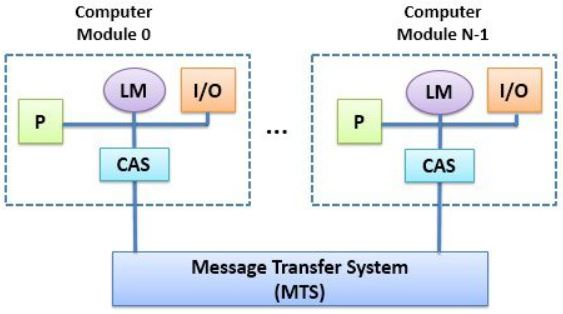
\includegraphics[width=8cm]{../img/loose}
\caption{A loosely coupled multiprocessor system. Each node features it's own memory and IO modules and uses a Message Transfer System to perform inter-node communication. Image source: \cite{preeti_aritra_2017}.}
\label{fig:loose}
\end{figure}
\end{minipage}
\begin{minipage}{0.05\textwidth}\hfill\end{minipage}
\begin{minipage}{0.45\textwidth}
\begin{figure}[H]
\centering
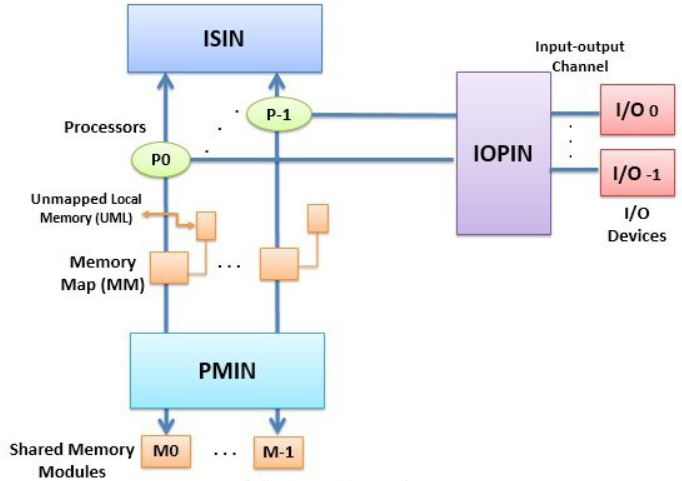
\includegraphics[width=8cm]{../img/tight}
\caption{A tightly coupled multiprocessor system. Nodes are directly connected to memory and IO modules. Image source: \cite{preeti_aritra_2017}.}
\label{fig:tight}
\end{figure}
\end{minipage}
\vspace{0.3cm}

This project will utilise a loosely coupled architecture due to it's easier scalability implementation and my previous experience with the design of single-core processors. Although it will require a scheduler to access the MTS, the experience and knowledge gained from this task will be greatly beneficial for future projects.

\section{Network-on-chip Architectures}
Network-on-chip (NoC) architectures implement on-chip communication mechanisms that are based on network communication  principles, such as routing, switching, and massive scalability \cite{newnoc}. NoC's can generally support hundreds to millions of processing cores.
\cref{fig:noc} shows an example 16-core network-on-chip architecture. 
NoC's can scale to very large sizes while not sacrificing performance because each processor core is able to drive the network rather than needing to wait for a shared bus to become free before doing so.

The greater the number of cores in a network-on-chip design, the greater quality of service (QoS) problems arise. As such, network-on-chip architectures suffer the same problems as networks, such as fairness and throughput \cite{nocfairness}.


\begin{figure}[h]
\centering
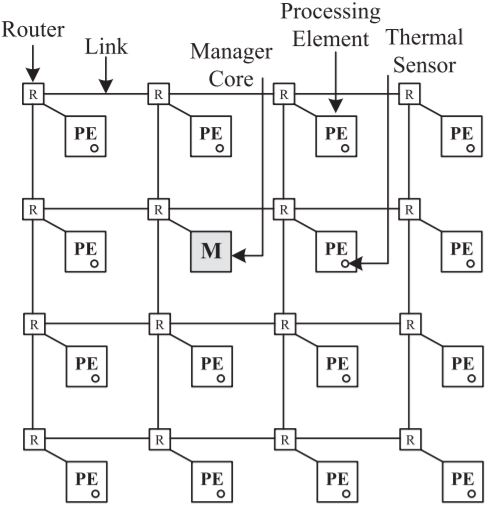
\includegraphics[width=6cm]{../img/noc}
\caption{A multiprocessor network-on-chip architecture with 16 processing nodes. Nodes are connected in a grid formation with routers and links. Image source: \cite{noc}.}
\label{fig:noc}
\end{figure}


\chapter{Project Overview}
{%\hypersetup{linkcolor=black}
\startcontents[chapters]
\printcontents[chapters]{}{1}{}
}
\noindent\\
This chapter discusses the the project's requirements, goals, and structure.

\section{Project Deliverables}
\label{sect:goals}
The project's deliverables are split into two sections: core deliverables (CD) -- each deliverable must be satisfied for the project to be a minimum viable product (MVP), and extended deliverables (ED) -- deliverables that are not required for a MVP -- features that only improve upon an existing feature.

\subsection{Core Deliverables (CD)}
The project's core deliverables are described below.
\begin{enumerate}[leftmargin=2\parindent, label=\bfseries CD\arabic*]
\item{\textbf{Design a compact 16-bit RISC instruction set architecture.}\\
The instruction set will be the primary interface to control the processor from software. An instruction set will be required to implement the custom multi-core communication interface.

It was decided to design a new instruction set rather than to extend an existing architecture as this will increase my knowledge of the constraints to consider when designing instruction sets and processors.
}
\label{cd:isa}

\item{\textbf{Design and implement a Verilog RISC core that implements the ISA in \ref{cd:isa}.}\\
The Verilog RISC core will be able to run software program written for the instruction set architecture.
}\label{cd:core}

\item{\textbf{Design and implement an on-chip interconnect for multi-core processing (2 to 32 cores) using the RISC core from \ref{cd:core}.}\\
The interconnect will be a chief requirement to enable multi-core communication. The interconnect should support up to 32 cores, however FPGA implementation constraints may limit this due to limited resources.

The interconnect will control communication between the cores to enable software parallelism.
}\label{cd:interconnect}

\item{\textbf{Analyse performance of serial and parallel software algorithms, such as parallel DFT, on the processor.}\\
To evaluate the effectiveness of the developed solution, a serial and parallel implementation of a simple computing algorithm (parallel reduction, sorting) will be ran on the processor and it's performance analysed. Effectiveness will be rated on total algorithm run-time and the speed-up gained by adding more cores.
}\label{cd:software}

\item{\textbf{Allow the RISC core to be easily compiled to multiple FPGA vendors (Xilinx, Altera).}\\
The developed solution should be generic and portable to allow it to be used across a wide-range of FPGA vendors and devices.

Verilog is a generic implementation-independent hardware-description language and so designing implementation specific modules is recommended.

A key consideration for this requirement is to consider the varying hard IP provided by the FPGA vendors (such as BRAM, ethernet, and PCIe \cite{xilinxbram,alterabram}). To overcome this problem, the developed Verilog code will conditionally compile where vendor specific requirements are present.
}\label{cd:vendor}
\end{enumerate}

\subsection{Extended Deliverables (ED)}
The project's extended deliverables are described below.
\begin{enumerate}[leftmargin=2\parindent, label=\bfseries ED\arabic*]
    \item{Design a RISC core with an instructions-per-clock (IPC) rating of at least 1.0 (a single-cycle CPU).}
\label{ed:ipc}
    \item{Design a RISC core with a pipe-lined data path to increase the design's clock speed.}\label{ed:pipeline}
    \item{Design a scalable multi-core interconnect supporting arbitrary (more than 32) RISC core instances (manycore) using Network-on-Chip (NoC) architecture.}\label{ed:scale}
    \item{Design a compiler-backend for the PRCO304 \cite{prco304} compiler to support the ISA from \ref{cd:isa}. This will make it easier to build complex multi-core software for the processor.}\label{ed:compiler}
    \item{The RISC core can communicate to peripherals via a memory-mapped addresses using the Wishbone bus.}\label{ed:mmu}
    \item{Implement various memory-mapped peripherals such as UART, GPIO, LCD, to aid visual representation of the processor during the demonstration viva.}\label{ed:peripherals} 
    \item{Store instruction memory in SPI flash.}\label{ed:flash}
    \item{Reprogram instruction memory at runtime from host computer.}\label{ed:program}
    \item{Processor external debugger using host-processor link.}\label{ed:debug}
\end{enumerate}

\section{Project Timeline}
\label{sect:timeline}
\subsection{Project Stages}
The project is split up into many stages to aid planning and management of the project. There are 8 unique stage areas: 1. Inital project conception; 2 Basic RISC core development; 3. Extended RISC core development; 4. Multi-core development; 5. Processor quality-of-life (QoL) improvements; 6. Compiler development; 7. Demo preparation, and 8. Final report.

The project stages are shown in Table \ref{tb:stages}.

\begin{table}[h]
    \small
    \begin{tabularx}{\textwidth}{|l|l|l|l|l|X|}
    \hline
    Stage & Title & Start Date & Days & Core & Applicable Deliverables
    \\ \specialrule{2pt}{-2pt}{0pt}
    1.0 & Research & Feb 04 & 7 & x & 
    \\ \hline
    1.1 & Requirement gathering/review & Feb 11 & 14 & x & 
	\\ \hline
    1.1 & Processor specification, architecture, ISA & Feb 18 & 100 & x & \ref{cd:isa}
	\\ \hline
    1.2 & Stage/Time Allocation Planning & Feb 25 & 7 & x & 
    \\ \specialrule{2pt}{-2pt}{0pt}
    2.1 & Decoder, Register Set, impl \& integration & Feb 25 & 14 & x & \ref{cd:core}
	\\ \hline
    2.2 & Register set impl \& integration & Mar 04 & 14 & x & \ref{cd:core}
	\\ \hline
    2.3 & Local memory impl \& integration & Mar 11 & 14 & x & \ref{cd:core}
    \\ \specialrule{2pt}{-2pt}{0pt}
    3.1 & Memory mapped register layout \& impl & Apr 01 & 21 &  & \ref{ed:mmu}
	\\ \hline
    3.2 & Wishbone peripheral bus connected to MMU & Apr 08 & 21 &  & \ref{ed:mmu}
	\\ \hline
    3.3 & Pipelined implementation and verification & Apr 15 & 21 &  & \ref{ed:pipeline}
	\\ \hline
    3.4 & Cache memory design \& impl & Apr 22 & 28 &  & \ref{ed:pipeline}
    \\ \specialrule{2pt}{-2pt}{0pt}
    4.1 & Multi-core communication interface & TBD & TBD & x & \ref{cd:interconnect}
	\\ \hline
    4.2 & Shared-memory controller & TBD & TBD & x & \ref{cd:interconnect}
	\\ \hline
    4.3 & Scalable multi-core interface (10s of cores) & TBD & TBD & x & \ref{cd:interconnect}
	\\ \hline
    4.4 & Multi-core example program (reduction) & TBD & TBD & x & \ref{cd:software}
    \\ \specialrule{2pt}{-2pt}{0pt}
    5.1 & SPI-FPGA interface for OTG programming & TBD & TBD &  & \ref{ed:flash}
	\\ \hline
    5.2 & FPGA-PC interfacing & TBD & TBD &  & \ref{ed:debug}
	\\ \hline
    5.3 & FPGA-PC debugging (instruction breakpoints) & TBD & TBD &  & \ref{ed:debug}
    \\ \specialrule{2pt}{-2pt}{0pt}
    6.1 & Compiler backend for vmicro16 & TBD & TBD &  & \ref{ed:compiler}
	\\ \hline
    6.2 & Compiler support for multi-core codegen & TBD & TBD &  & \ref{ed:compiler}
    \\ \specialrule{2pt}{-2pt}{0pt}
    7.1 & Wishbone peripherals for demo & TBD & TBD & x & \ref{cd:software}
    \\ \specialrule{2pt}{-2pt}{0pt}
    8.1 & Final Report & TBD & TBD & x & 
	\\ \hline
    \end{tabularx}
    \caption{Project stages throughout the life cycle of the project.}
    \label{tb:stages}
\end{table}

\subsection{Project Stage Detail}
\subsubsection{Stages 1.0 through 1.2 --  Research and Project Conception}
These stages cover initial research of existing problems and solutions in the multiprocessor area. 
The instruction set architecture is also proposed that later stages will implement.

\subsubsection{Stages 2.1 through 2.3 -- Processor module Design, Implementation, and Integration}
These stages cover the design, implementation, and integration of key processor core modules such as the instruction decoder, register sets and local memory.
Integration of all the modules is a challenging task because some modules have both asynchronous and synchronous signals that need to be timed correctly in order for other modules to receive valid data. An example of this is the register set which has asynchronous read ports that are later clocked in the instruction decode stage.

\subsubsection{Stages 3.1 through 3.4 -- Advanced Processor Implementation}
These stages add advanced features to the processor to provide a more functional product. Although these stages are classified as extended, their technical requirement to design and implement is not great and so are have time allocations in the project schedule. The extended features that these stages introduce are: pipelined processor stages -- to drastically increase processor performance; provide a memory-mapped peripheral interface through the MMU; provide a Wishbone master interface to the MMU -- allowing external peripherals such as GPIO and LCD displays to be utilised in a modular fashion; and to implement a cache memory for each processor core.

\subsubsection{Stages 4.1 through 4.4 -- Multiprocessor Functionality}
These stages are dedicated to adding multiprocessor functionality using a loosely coupled architecture to the processor.

\subsubsection{Stages 5.1 through 5.3 -- Debugging Features}
These stages cover debugging features and are classified as extended due to the large development time required to implement them as well as not being related to multiprocessor systems.

\subsubsection{Stages 6.1 through 6.2 -- Compiler Backends}
These stages cover the implementation of a compiler backend to ease software writing and programming of the processor.

\subsubsection{Stage 7.1 -- Wishbone Peripherals}
Additional Wishbone peripherals, such as SPI and timers will be added to produce a more useful multiprocessor system.

\subsubsection{Stage 8.1 -- Final Report}
This stage is dedicated to the final report write-up. It is expected to be an iterative task that is active throughout the lifespan of the project.

\subsection{Timeline}
The project stages from Table \ref{tb:stages} are displayed below in a Gantt chart.

\begin{figure}[h]
\centering
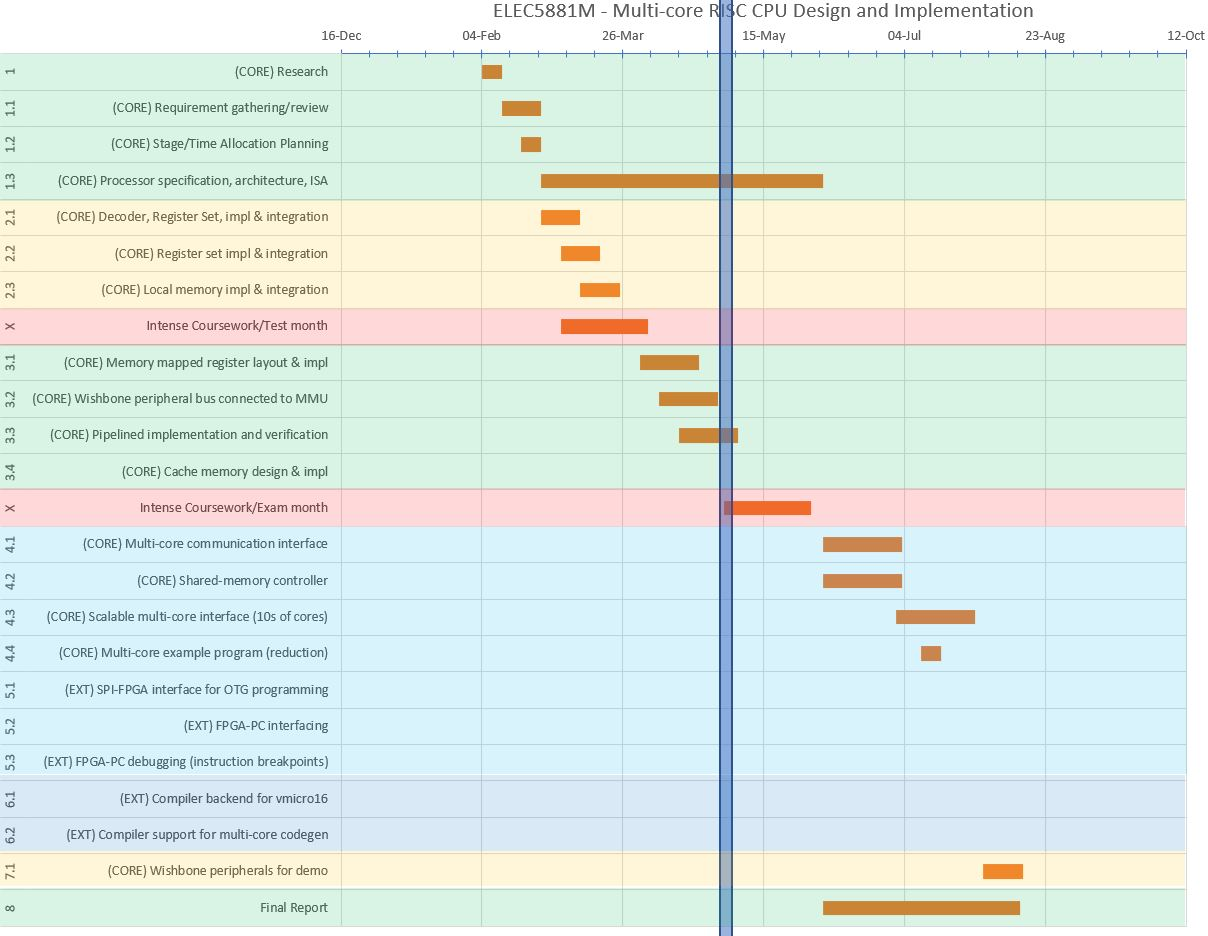
\includegraphics[width=13cm]{../img/week2_gantt}
\caption{Project stages in a Gantt chart.}
\label{fig:gantt}
\end{figure}


\section{Resources}
This section describes the hardware and software resources required to fulfil the project. 

\subsection{Hardware Resources}
Core deliverable \ref{cd:vendor} requires the designed RISC core to be implemented and demonstrated on multiple FPGA devices.  Although my design should synthesise for physical IC implementation, due to high costs and lengthy production times, it is not a primary development target. 
Due to having past experience with Xilinx FPGAs from my placement work and experience with Altera from university modules it was decided to target the Xilinx Spartan 6 XC6SLX9 and the Altera Cyclone V.

\subsubsection{Terasic DE1-SoC Development Board}
The Terasic DE1-SoC development board features a large Cyclone V FPGA and many peripherals, such as seven-segment displays, 64 MB SDRAM, ADCs, and buttons and switches, which will aid demonstration of the project. The development board is available through the university so the cost is negligible. \cref{fig:de1soc} shows the peripherals (green) available to the FPGA.

\begin{figure}[h]
\centering 
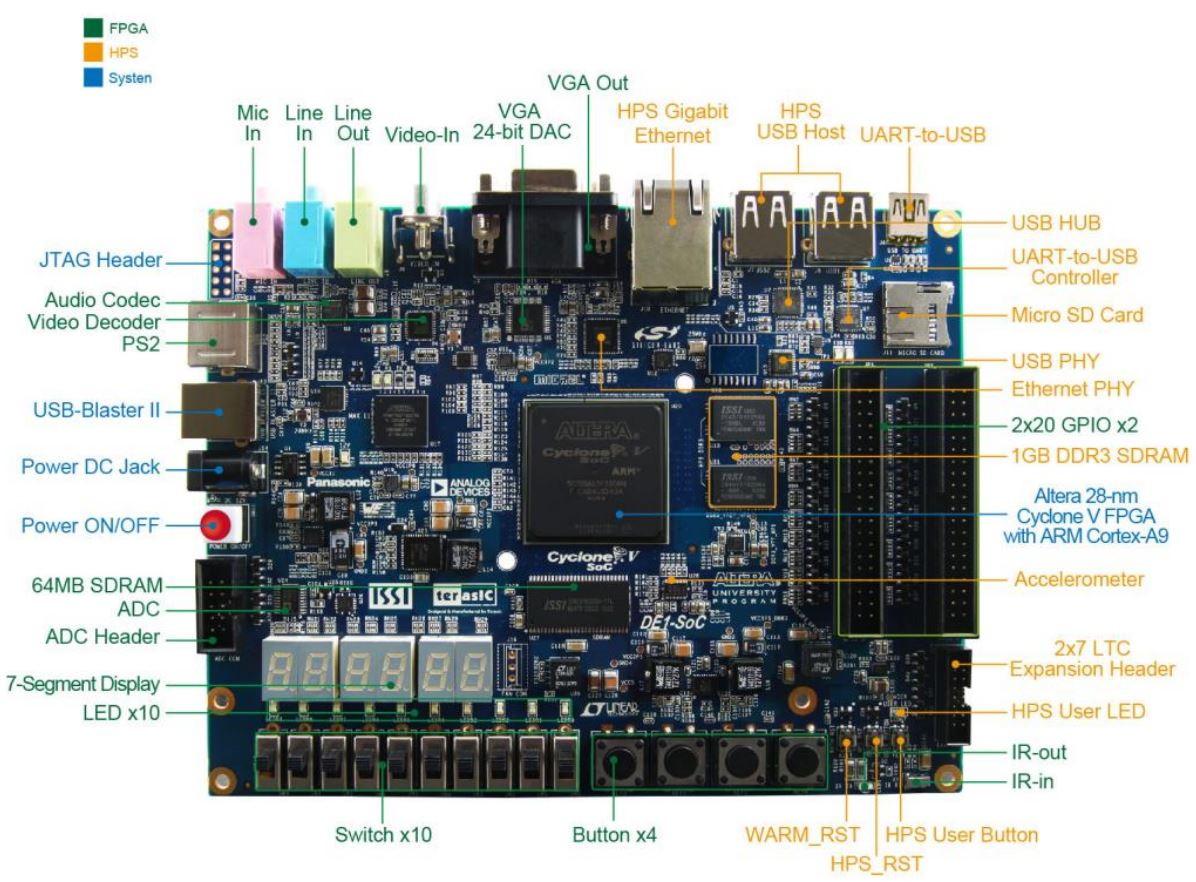
\includegraphics[width=10cm]{../img/de1soc}
\caption{Terasic DE1-SoC development board featuring the Altera Cyclone V FPGA and many peripherals. Image source: \cite{de1soc}.}
\label{fig:de1soc}
\end{figure}

\subsubsection{Minispartan 6+ FPGA Development Board}
The Minispartan 6+ is a hobbyist FGPA development board with fewer peripherals than the DE1-SoC. The board features a Xilinx Spartan 6 XC6LX9 which has far fewer resources than the DE1-SoC's Cyclone V however it's simplicity and my familiarity with  Xilinx's software suite will speed up development. The development board is shown in \cref{fig:minispartan}.

\begin{figure}[h]
\centering 
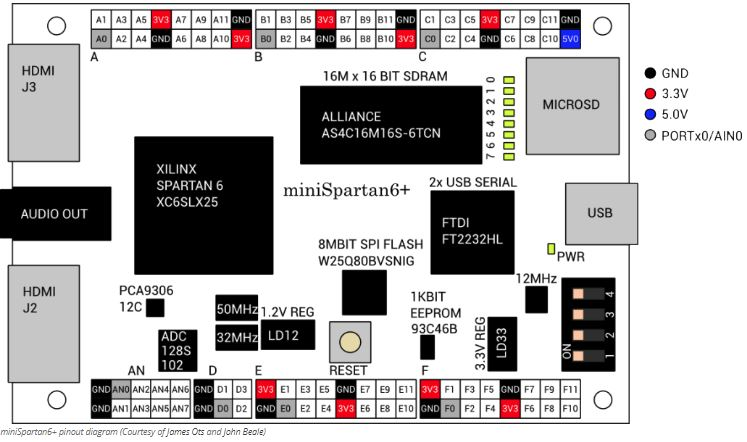
\includegraphics[width=10cm]{../img/minispartan}
\caption{Minispartan-6+ development board featuring the Xilinx Spartan 6 XC6SLX9. Note that the XC6SLX9 and XC6SLX25 FPGAs share the same board. Image source: \cite{scarabhardware}.}
\label{fig:minispartan}
\end{figure}

\subsection{Software Resources}
\subsubsection{Intel Quartus}
Intel Quartus Prime is a paid-for SoC, CPLD, and FPGA software suite targeting Intel's Stratix, Arria, and Cyclone based FPGAs. The university provides student licences which will be used via VPN.


\subsubsection{Xilinx ISE Webpack}
Xilinx ISE Webkpack is Xilinx's free software suite for FPGA development for Spartan 6 based FPGAs.
Due to ISE's intuitive and fast work flow, most of the initial simulation and verification processes will be performed using ISE. This will greatly improve development times.

\subsubsection{Verilator}
Verilator is an open-source Verilog to C++ transpiler which provides a C++ interface to simulate Verilog modules and read/write values similar to a test bench. Verilator will be used for specific modules within the RISC core such as the ALU and decoder as Verilator is useful when performing exhaustive verification.

\section{Legal and Ethical Considerations}
The RISC core is designed to be used as an academic research and educational tool to aid learning and understanding of RISC and multi-core machines. It should not be use for roles where mission critical or safety is a factor. 

The processor does not provide any memory protection features and any software running on the processor has full access to all memory.

The processor does not store/track/predict software instructions. The processor uses pipelining techniques to improve performance which results in future instructions entering the pipeline even if the software's logical sequence does not include these instructions. This could result in security vulnerabilities similar to Intel's Spectre vulnerability \cite{kocher2018spectre}.


\chapter{Single-core Design}
\startcontents[chapters]
\printcontents[chapters]{}{1}{}

\section{Introduction}
While the majority of this report will focus on the multi-processing functionality of this project, it is important understand the design decisions of the single core to understand the features and limitations of the multi-core system-on-chip as a whole.

\section{Design and Implementation}
The single-core design is a traditional 5-stage RISC processor (fetch, decode, execute, memory, write-back). The core uses separate instruction and data memories in the style of a Harvard architecture \cite{harvard}.

To satisfy \ref{cd:vendor}, the Verilog code will be self-contained in a single file. This reduces the hierarchical complexity and eases cross-vendor project set-up as only a single file is required to be included. 
A disadvantage with this single file approach is that some external Verilog verification tools that I plan to use, such as Verilator, do not currently support multiple Verilog modules (due to an unfixed bug) within a single file. 

\begin{figure}[H]
\centering 
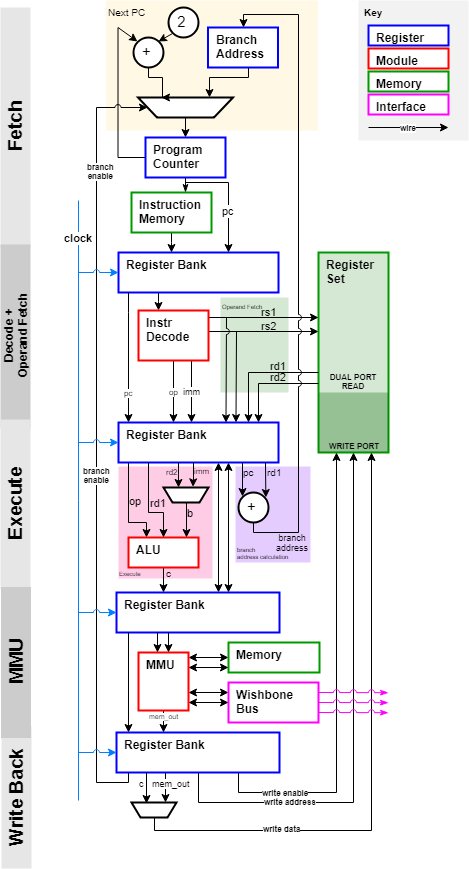
\includegraphics[width=10cm]{../img/risc}
\caption{Vmicro16 RISC 5-stage RTL diagram showing: instruction pipelining (data passed forward through clocked register banks at each stage); branch address calculation; ALU operand calculation (rd2 or imm); and program counter incrementing.}
\label{fig:risc}
\end{figure}

A small reduction in size within the single-core will result in substantial size reductions in 

\subsection{Instruction Set Architecture}
\begin{quotation}
\noindent Core deliverable \ref{cd:isa} details the background for the requirement of a custom instruction set architecture.
\end{quotation}

\noindent
The 16-bit instruction set listing is shown in \cref{fig:isa}.

Most instructions are \textit{destructive}, meaning that source operands also act as the destination, hence effectively \textit{destroying} the original source operand. This design decision reduces the complexity of the ISA as traditional three operand instructions, for example \verb|add r0, r0, r1|, can be encoded using only two operands \verb|add r0, r1|. However, this does increase the complexity of compilers as they may need to make temporary copies of registers as the instructions will \textit{destroy} the original data.

The instruction set is split into 7 categories (highlighted by colours in \cref{fig:isa}): special instructions, such as halting and interrupt returns; memory operations, such as loading and storing; bitwise operations, such as XOR and AND; unsigned arithmetic; signed arithmetic; conditional branches; and atomic load/store instructions.

%The instruction set supports bitwise operations such as OR, XOR, AND, NOT, and left and right shifts. It was decided to provide these functions to enable software to easily create large 16-bit values which is expensive with only an 8-bit immediate.

\subsection{Instruction and Data Memory}
The design uses separate instruction and data memories similar to a Harvard architecture computer. This architecture was chosen due because it is generally easier to implement, however later resulted in design challenges in large multi-core designs. This is discussed later in the report.

\subsection{Memory Management Unit}
It was decided to use a memory management unit (MMU) to make it easier and extensible to communicate with external peripherals or additional registers. This method would transparently use the existing \verb|LW|/\verb|SW| instructions which removes the requirement for a unique instruction for each peripheral. 


\subsection{ALU Design}
The Vmicro16's ALU is an asynchronous module that has 3 inputs: data a; data b; and opcode op; and outputs data c.
The ALU is able to operate on both register data (\verb|rd1| and \verb|rd2|) and immediate values. A switch is used to set the \verb|b| input to either the \verb|rd2| or \verb|imm| value from the previous stage.

\begin{figure}[H]
\centering 
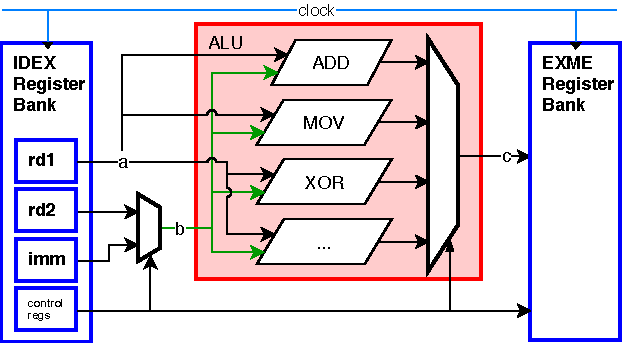
\includegraphics[width=10cm]{../img/alu}
\caption{Vmicro16 ALU diagram showing clocked inputs from the previous IDEX stage being }
\label{fig:alu}
\end{figure}

The ALU also performs comparison (\verb|CMP|) operations in which it returns flags similar to X86's overflow, signed, and zero, flags. The combination of these flags can be used to easily compute relationships between the two input operands. For example, if the zero flag is not equal to the signed flag, then the relationship between inputs $a$ and $b$ is that $a < b$.

\begin{listing}[H]
\centering
\begin{minted}[fontsize=\scriptsize,linenos,baselinestretch=0.5,frame=single,framesep=10pt]{verilog}
module branch (
    input [3:0] flags,
    input [7:0] cond,
    output reg  en
);
    always @(*)
        case (cond)
            `VMICRO16_OP_BR_U:  en = 1;
            `VMICRO16_OP_BR_E:  en = (flags[`VMICRO16_SFLAG_Z] == 1);
            `VMICRO16_OP_BR_NE: en = (flags[`VMICRO16_SFLAG_Z] == 0);
            `VMICRO16_OP_BR_G:  en = (flags[`VMICRO16_SFLAG_Z] == 0) && 
                                     (flags[`VMICRO16_SFLAG_N] == flags[`VMICRO16_SFLAG_V]);
            `VMICRO16_OP_BR_L:  en = (flags[`VMICRO16_SFLAG_Z] != flags[`VMICRO16_SFLAG_N]);
            `VMICRO16_OP_BR_GE: en = (flags[`VMICRO16_SFLAG_Z] == flags[`VMICRO16_SFLAG_N]);
            `VMICRO16_OP_BR_LE: en = (flags[`VMICRO16_SFLAG_Z] == 1) || 
                                     (flags[`VMICRO16_SFLAG_N] != flags[`VMICRO16_SFLAG_V]);
            default:            en = 0;
        endcase
endmodule
\end{minted}
\caption{ALU branch detection using flags: zero (Z), overflow (V), and negative (N).}
\end{listing}


The Verilog implementation of the ALU is shown in \cref{fig:aluv}. The ALU's asynchronous output is clocked with other registers, such as destination register \verb|rs1| and other control signals, in the \verb|EXME| register bank.
\begin{listing}[H]
\centering
\begin{minted}[fontsize=\scriptsize,linenos,baselinestretch=0.5,frame=single,framesep=10pt]{verilog}
always @(*) case (op)
    // branch/nop, output nothing
    `VMICRO16_ALU_BR,
    `VMICRO16_ALU_NOP:          c = {DATA_WIDTH{1'b0}};
    // load/store addresses (use value in rd2)
    `VMICRO16_ALU_LW,
    `VMICRO16_ALU_SW:           c = b;
    // bitwise operations
    `VMICRO16_ALU_BIT_OR:       c = a | b;
    `VMICRO16_ALU_BIT_XOR:      c = a ^ b;
    `VMICRO16_ALU_BIT_AND:      c = a & b;
    `VMICRO16_ALU_BIT_NOT:      c = ~(b);
    `VMICRO16_ALU_BIT_LSHFT:    c = a << b;
    `VMICRO16_ALU_BIT_RSHFT:    c = a >> b;
\end{minted}
\caption{Vmicro16's ALU implementation named vmicro16\_alu. vmicro16.v}
\label{fig:aluv}
\end{listing}




\subsection{Decoder Design}
Instruction decoding occurs in the between the IFID and IDEX stages. 
The decoder extracts register selects and operands from the input instruction. The decoder outputs are asynchronous which allows the register selects to be passed to the register set and register data to be read asynchronously. The register selects and register read data is then clocked into the IDEX register bank.

\begin{listing}[H]
\centering
\begin{minted}[fontsize=\scriptsize,linenos,baselinestretch=0.5,frame=single,framesep=10pt]{verilog}
always @(*) case (instr[15:11])
    `VMICRO16_OP_BR:              alu_op = `VMICRO16_ALU_BR;
    `VMICRO16_OP_MULT:            alu_op = `VMICRO16_ALU_MULT;

    `VMICRO16_OP_CMP:             alu_op = `VMICRO16_ALU_CMP;
    `VMICRO16_OP_SETC:            alu_op = `VMICRO16_ALU_SETC;
    
    `VMICRO16_OP_BIT:     casez (instr[4:0])
        `VMICRO16_OP_BIT_OR:      alu_op = `VMICRO16_ALU_BIT_OR;
        `VMICRO16_OP_BIT_XOR:     alu_op = `VMICRO16_ALU_BIT_XOR;
        `VMICRO16_OP_BIT_AND:     alu_op = `VMICRO16_ALU_BIT_AND;
        `VMICRO16_OP_BIT_NOT:     alu_op = `VMICRO16_ALU_BIT_NOT;
        `VMICRO16_OP_BIT_LSHFT:   alu_op = `VMICRO16_ALU_BIT_LSHFT;
        `VMICRO16_OP_BIT_RSHFT:   alu_op = `VMICRO16_ALU_BIT_RSHFT;
        default:                  alu_op = `VMICRO16_ALU_BAD; endcase
\end{minted}
\caption{Vmicro16's ALU implementation named vmicro16\_alu. vmicro16.v}
\caption{Vmicro16's decoder module code showing nested bit switches to determine the intended opcode. vmicro16.v}
\label{fig:vdecoder}
\end{listing}

In \cref{fig:vdecoder}, it can be seen that the first 4 opcode cases (BR, MULT, CMP, SETC) are represented using the same 15-11 (opcode) bits, however the BIT instructions share the same opcode and so require another bit range to be compared to determine the output function.



\subsection{Pipelining}
In the interim progress update, the processor design featured \textit{instruction pipelining} to meet requirement \ref{ed:ipc}. Instruction pipelining allows instructions executions to be overlapped in the pipeline, resulting in higher throughput (up to one instruction per clock) at the expense of 5-6 clocks of latency and code complexity. As the development of the project shifted from single-core to multi-core, it became obvious that the complexity of the pipelined processor would inhibit the integration of multi-core functionality. It was decided to remove the instruction pipelining functionality and use a simpler state-machine based pipeline that is much simpler to extend and would cause fewer challenges later in the project. 

\subsection{Design Optimisations}
In a design that has many instantiations of the same component, a small resource saving improvement within the component can have a significant overall savings improvement if it is instantiated many times. Project requirement \ref{cd:vendor} requires the design to be compiled for a range of FPGA sizes, and so space saving optimisations are considered. 

\subsubsection{Register Set Size Improvements}
A register set in a CPU is a fast, temporary, and small memory that software instructions directly manipulate to perform computation. In the Vmicro16 instruction set, eight registers named r0 to r7 are available to software. The instruction set allows up to two registers to be references in most instructions, for example the instruction \verb|add r0, r1| tells the processor to perform the following actions:
\begin{enumerate}[leftmargin=4\parindent, label=\bfseries Clock \arabic*.]
\item Fetch r0 and r1 from the register set
\item Add the two values together in the ALU
\item Store the result back the register set in r0
\end{enumerate}
For task 1, it was originally decided to use a dual port register set (meaning that two data reads can be performed in a single clock, in this case r0 and r1), however due to the asynchronous design of the register set (for speed) the RTL produced consumed a significant amount of FPGA resources, approximately 256 flip-flops (16 (data width) * 8 (registers) * 2 (ports)). To reduce this, it was decided to split task 1 into two steps over two clock cycles using a single-port register set. This required the processor pipe-line to use another clock cycle resulting in slightly lower performance, however the size improvements will allow for more cores to be instantiated in the design. This optimisation is also applied to the interrupt register set, resulting in a saving of approximately 256 flip-flops per core (128 in the normal mode register set, and 128 in the interrupt register set). As shown, adding a single clock delay saves a significant amount of LUTs. This saving is amplified when instantiating many cores.



\section{Interrupts}
\label{sect:interrupts}
Interrupts are a technique used by processors to run software functions when an event occurs within the processor, such as exceptions, or signalled from an external source, such as a UART receiver signalling it has received new data. Today, it is common for micro-controllers, soft-processors, and desktop processors, to all feature interrupts. Modern implementations support an \textit{interrupt vector} which is a memory array that contains addresses to different \textit{interrupt handlers} (a software function called when a particular interrupt is received).

Although interrupts are not a requirement for a multi-core system, it was decided to implement this functionality to boost my understanding of such systems. In addition, example demos provided with this project are better visualised with a interrupt functionality.

The interrupt functionality in this project supports the following:
\begin{itemize}
\item Per-core 8 cell interrupt vector accessible to software.\\Software programs running on the Vmicro16 processor can edit the interrupt vector to /
\end{itemize}

\subsection{Hardware Implementation}

\subsubsection{Context Switching}
When acting upon an incoming interrupt the current state the processor must be saved so that changes from the interrupt handler, such as register writes and branches, do not affect the current state. After the interrupt handler function signals it has finished (by using the \textit{Interrupt Return} \verb|INTR| instruction) the saved state is restored.
In the case of the Vmicro16 processor, the program counter \verb|r_pc[15:0]| and register set \verb|regs| instance are the only states that are saved. Going forth, the terms \textit{normal mode} and \textit{interrupt mode} are used to describe what registers the processor should use when executing instructions.

When saving the state, to avoid clocking 128 bits (8 registers of 16 bits) into another register (which would increase timing delays and logic elements), a dedicated register set for the interrupt mode (\verb|regs_isr|) is multiplexed with the normal mode register set (\verb|regs|). Then depending on the mode (identified by the register \verb|regs_use_int|) the processor can easily switch between the two large states without significantly affecting timing.

The timing diagram in \cref{fig:interrupts} visually describes this process.

\begin{figure}[h]
\centering
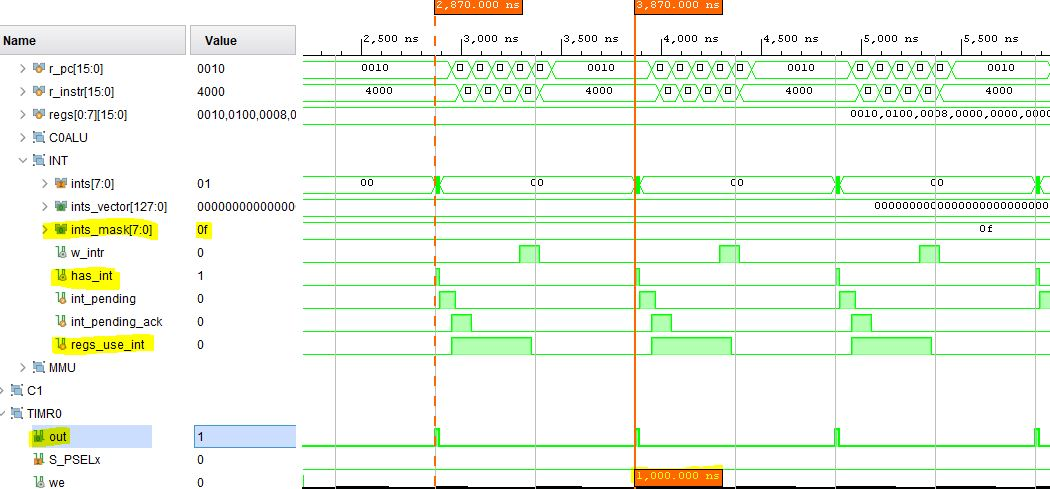
\includegraphics[width=\textwidth]{interrupts}
\caption{Time diagram showing the TIMR0 peripheral emitting a 1us periodic interrupt signal (out) to the processor. The processor acknowledges the interrupt (int\_pending\_ack) and enters the interrupt mode (regs\_use\_int) for a period of time. When the interrupt handler reaches the Interrupt Return instruction (indicated by w\_intr) the processor returns to normal mode and restores the normal state.}
\label{fig:interrupts}
\end{figure}

\subsection{Software Interface}
To enable software to 

\begin{figure}[H]
\centering
\begin{bytefield}[bitwidth=4ex, rightcurly=., rightcurlyspace=0pt]{16}
\bitheader[endianness=big]{0-15} \\
\begin{rightwordgroup}{0100 RW}
\bitbox{16}{Interrupt handler $0$}
\end{rightwordgroup} \\

\bitbox[]{16}{$\vdots$ \\[1ex]} \\
\begin{rightwordgroup}{0107 RW}
\bitbox{16}{Interrupt handler $7$}
\end{rightwordgroup} \\

\begin{rightwordgroup}{0108 RW}
\bitbox{8}{\color{lightgray}\rule{\width}{\height}} & \bitbox{8}{Interrupt bit mask}
\end{rightwordgroup}
\end{bytefield}
\caption{The interrupt vector consists of eight 16-bit values that point to memory addresses of the instruction memory to jump to.}
\label{fig:r_interrupts}
\end{figure}

\subsubsection{Interrupt Vector (0x0100-0x0107)}
The interrupt vector is a per-core register that is used to store the addresses of interrupt handlers. An interrupt handler is simply a software function residing in instruction memory that is branched to when a particular interrupt is received. 

\subsubsection{Interrupt Mask (0x0108)}
The interrupt mask is a per-core register that is used to mask/listen specific interrupt sources. This enables processing cores to individually select which interrupts they respond to. This allows for multi-processor designs where each core can be used for a particular interrupt source, improving the time response to the interrupt for time critical programs. The Interrupt Mask register is an 8-bit read/write register where each bit corresponds to a particular interrupt source and each bit corresponds with the interrupt handler in the interrupt vector.

\begin{figure}
\centering
\begin{bytefield}[bitwidth=4ex]{16}
& \bitlabel{8}{} &
& \bitlabel{6}{[7:2] User defined} &
& \bitlabel{1}{UART0 RX} 
& \bitlabel{1}{TIMR0} \\
\bitheader[endianness=big]{0-7,8,15} \\
  \bitbox{8}{\color{lightgray}\rule{\width}{\height}}
& \bitbox{1}{0}
& \bitbox{1}{0}
& \bitbox{1}{0}
& \bitbox{1}{0}
& \bitbox{1}{0}
& \bitbox{1}{0}
& \bitbox{1}{0}
& \bitbox{1}{0}
\end{bytefield}
\caption{Interrupt Mask register (0x0108). Each bit corresponds to an interrupt source. 1 signifies the interrupt is enabled for/visible to the core. Bits [7:2] are left to the designer to assign.}
\label{fig:r_interruptmask}
\end{figure}

\subsubsection{Software Example}
To better understand the usage of the described interrupt registers, a simple software program is described below. The following software program produces a simple and power efficient routine to initialise the interrupt vector and interrupt mask.

% pip install pygments-arm
\begin{minted}[fontsize=\footnotesize,linenos,,baselinestretch=0.8]{arm}
entry:
    // Set interrupt vector at 0x100
    // Move address of isr0 function to vector[0]
    movi    r0, isr0
    // create 0x100 value by left shifting 1 8 bits
    movi    r1, #0x1
    movi    r2, #0x8
    lshft   r1, r2
    // write isr0 address to vector[0]
    sw      r0, r1
    
    // enable all interrupts by writing 0x0f to 0x108
    movi    r0, #0x0f
    sw      r0, r1 + #0x8
    halt                  // enter low power idle state
    
isr0:                     // arbitrary name
    movi    r0, #0xff     // do something
    intr                  // return from interrupt
\end{minted}

A more complex example software program utilising interrupts and the TIMR0 interrupt is described in section \ref{sect:timr0_code}.

\subsection{Design Improvements}
The hardware and software interrupt design have changed throughout the projects cycle. In initial versions of the interrupt implementation, the software program, while waiting for an interrupt, would be in a tight infinite loop (branching to the same instruction). This resulted in the processor using all pipeline stages during this time. The pipeline stages produce many logic transitions and memory fetches which raise power consumption and temperatures. This is quite noticeable especially when running on the Spartan-6 LX9 FPGA.

To improve this, it was decided to implement a new state within the processor's state machine that, when entered, did not produce high frequency logic transitions or memory fetches. The \verb|HALT| instruction was modified to enter this state and the only way to leave is from an interrupt or top-level reset. This removes the need for a software infinite loop that produces high frequency logic transitions (decoding, ALU, register reads, etc.) and memory fetches.





\section{Verification}
Various verification techniques are employed to ensure correct operation of the processor.

The first technique involves using static assertions to identify incorrect configuration parameters at compile time, such as having zero instruction memory and scratch memory depth. These assertions use the \verb|static_assert| for top level checks and \verb|static_assert_ng| for checks inside \verb|generate| blocks.

The second verification technique is to use assertions in \verb|always| blocks to identify incorrect behavioural states. This is done using the \verb|rassert| (run-time assert) macro.

The third verification technique is to use automatic verifying test benches. These test benches drive components of the processor, such as the ALU and decoder, and check the output against the correct value. This uses the \verb|rassert| macro.

The final method of verification is to verify the complete design via a behavioural test bench. The design is passed a compiled software program with a known expected output, and is ran until the \verb|r_halt| signal is raised. The test bench then checks the value on the \verb|debug0|, \verb|debug1|, and \verb|debug2| signals against the expected value. If this matches, then it is assumed that sub-components of the design also operate correctly. This technique does not monitor the states of sub-components and statistics (such as time taken to execute an instruction), there leaves the possibility that some components could have entered an illegal state.







\newpage
\chapter{Interconnect}
{%\hypersetup{linkcolor=black}
\startcontents[chapters]
\printcontents[chapters]{}{1}{}
}

%\noindent\\
%\lipsum[1]

\section{Introduction}
The Vmicro16 processor needs to communicate with multiple peripheral modules (such as UART, timers, GPIO, and more) to provide useful functionality for the end user.

Previous peripheral interface designs of mine have been directly connected to a main driver with unique inputs and outputs that the peripheral required. For example, a timer peripheral would have dedicated wires for it's load and prescaler values, wires for enabling and resetting, and wires for reading. A memory peripheral would have wires for it's address, read and write data, and a write enable signal. This resulted in each peripheral having a unique interface and unique logic for driving the peripheral, which consumed significant amounts of limited FPGA resources.

It can be seen that many of the peripherals need similar inputs and outputs (for example read and write data signals, write enables, and addresses), and because of this, a standard interface can be used to interface with each peripheral. Using a standard interface can reduce logic requirements as each peripheral can be driven by a single driver.

\subsection{Comparison of On-chip Buses}
The choice of on-chip interconnect has changed multiple times over the life-cycle of this project, primary due to ease of implementation and resource requirements. 

Originally, it was planned to use the Wishbone bus \cite{wishbone} due to it's popularity within open-source FPGA modules and good quality documentation.

Late in the project, it was decided to use the AMBA APB protocol \cite {ambaapb} as it is more commonly used in large commercial designs and understanding how the interface worked would better benefit myself. APB describes an intuitive and easy to implement 2-state interface aimed at communicating with low-throughput devices, such as UARTs, timers, and watchdogs.

\begin{figure}[H]
\centering
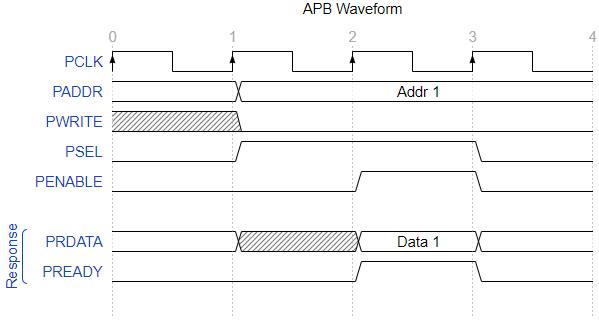
\includegraphics[width=0.7\textwidth]{apb_wave}
\caption{Waveform showing an APB read transaction.}
\end{figure}

\section{Overview}
The system-on-chip design is split into 3 main parts: peripheral interconnect (red), CPU array (gray), and the instruction memory interconnect (green).

A block diagram of this project is shown in Figure \ref{fig:watchdog}
\begin{figure}[H]
\centering
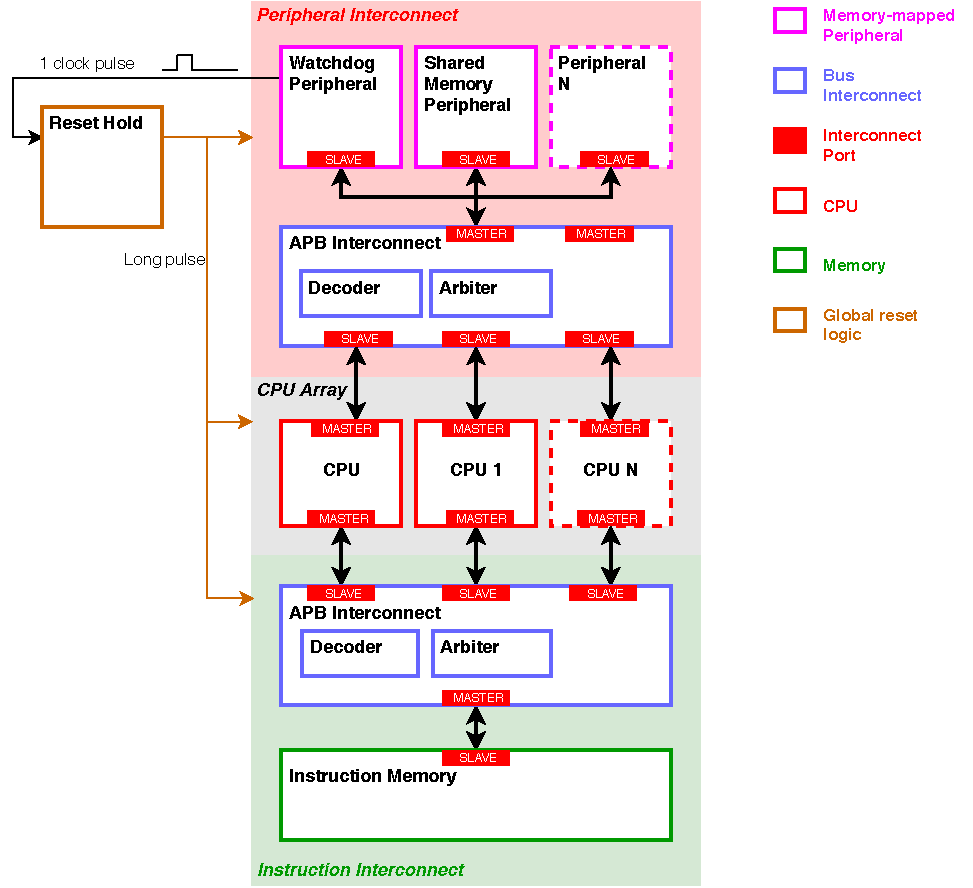
\includegraphics[width=\textwidth]{watchdog}
\caption{Block diagram of the Vmicro16 system-on-chip.}
\label{fig:watchdog}
\end{figure}

\subsection{Design Considerations}
There are several design issues to consider for this project. These are listed below:

\begin{itemize}
\item \textbf{Design size limitations}\\
The target devices for this project are small to medium sized FPGAs (featuring approximately 10,000 to 30,000 logic cells). Because of this, it is important to use a bus interconnect that has a small logic footprint yet is able to scale reasonably well.

\item \textbf{Ease of implementation}\\
The interconnect and any peripherals should be easy to implement within a reasonable time.

\item \textbf{Scalable}\\
The interconnect should allow for easy scalability of master and slave interfaces with minimal code changes.
\end{itemize}

\section{Interfaces}

\begin{figure}[H]
\centering
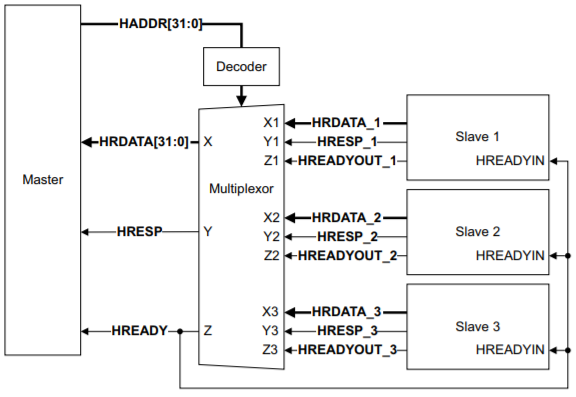
\includegraphics[width=0.7\textwidth]{ahb}
\end{figure}

\subsection{Master to Slave Interface}
\begin{figure}[H]
\centering
\begin{bytefield}[bitwidth=4ex, rightcurly=., rightcurlyspace=0pt]{21}
\bitheader[endianness=big]{0,15,16-20} \\
\begin{rightwordgroup}{PADDR[20:0]}
  \bitbox{1}{\rotatebox{90}{\small LE}}
  \bitbox{1}{\rotatebox{90}{\small SE}}
& \bitbox{3}{\small CORE\_ID}
& \bitbox{16}{Address}
\end{rightwordgroup}\\

\begin{rightwordgroup}{PWDATA[15:0]}
\bitbox{5}{\color{lightgray}\rule{\width}{\height}} & \bitbox{16}{Write data}
\end{rightwordgroup}\\

\begin{rightwordgroup}{PRDATA[15:0]}
\bitbox{5}{\color{lightgray}\rule{\width}{\height}} & \bitbox{16}{Read Data}
\end{rightwordgroup}\\

\begin{rightwordgroup}{PWRITE[0:0]}
\bitbox{20}{\color{lightgray}\rule{\width}{\height}} & \bitbox{1}{\rotatebox{90}{\small WE}}
\end{rightwordgroup}\\

\begin{rightwordgroup}{PENABLE[0:0]}
\bitbox{20}{\color{lightgray}\rule{\width}{\height}} & \bitbox{1}{\rotatebox{90}{\small EN}}
\end{rightwordgroup}
\end{bytefield}
\end{figure}

\newpage
\subsection{Multi-master Support}
\subsubsection{Design Goals}
\begin{enumerate}[leftmargin=3\parindent,label=\bfseries DG\arabic*.]
\item \textbf{Foo}\\
Bing
\end{enumerate}

\begin{figure}[h]
\centering
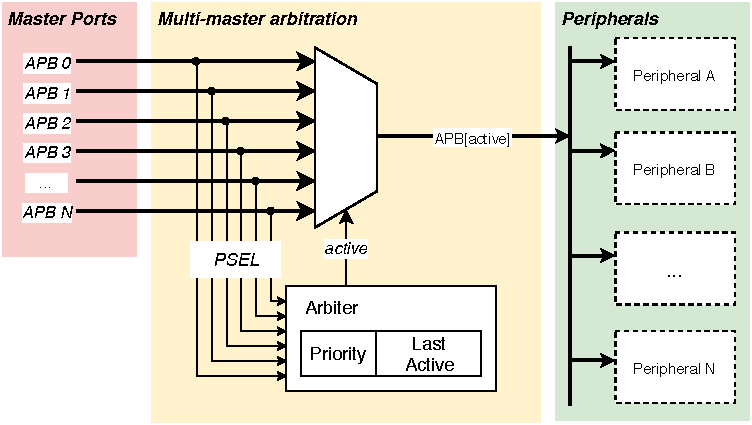
\includegraphics[width=\textwidth]{multimaster}
\caption{Foo}
\label{fig:multimaster}
\end{figure}


\begin{figure}[H]
\centering
\begin{minted}[fontsize=\footnotesize]{verilog}
input      [MASTER_PORTS*BUS_WIDTH-1:0]  S_PADDR,
input      [MASTER_PORTS-1:0]            S_PWRITE,
input      [MASTER_PORTS-1:0]            S_PSELx,
input      [MASTER_PORTS-1:0]            S_PENABLE,
input      [MASTER_PORTS*DATA_WIDTH-1:0] S_PWDATA,
output reg [MASTER_PORTS*DATA_WIDTH-1:0] S_PRDATA,
output reg [MASTER_PORTS-1:0]            S_PREADY,
\end{minted}
\caption{Variable size inputs and outputs to the interconnect.}
\end{figure}

\begin{figure}[H]
\centering
\begin{bytefield}[bitwidth=.5em, rightcurly=., rightcurlyspace=0pt]{84}
\bitheader[endianness=big]{0,20,41,62,83} \\
\bitbox{21}{Core $N$-$1$} & 
\bitbox{21}{$\cdots$} & 
\bitbox{21}{Core 1} & 
\bitbox{21}{Core 0}
\end{bytefield}
\end{figure}


\section{Further Work}
The submitted design is acceptable for a multi-core system as it fulfils the following requirements:
\begin{itemize}
\item Support an arbitrary number of peripherals.
\item Supports memory-mapped address decoding.
\item Supports multiple master interfaces.
\end{itemize}

\chapter{Memory Mapping}
{%\hypersetup{linkcolor=black}
\startcontents[chapters]
\printcontents[chapters]{}{1}{}
}
\noindent\\
The Vmicro16 processor uses a memory-mapping scheme to communicate with peripherals and other cores. This chapter describes the design decisions and implementation of the memory-map used in this project.

\section{Introduction}
Memory mapping is a common technique used by CPUs, micro-controllers, and other system-on-chip devices, that enables peripherals and other devices to be accessed via a memory address on a common bus. In a processor use-case, this allows for the reuse of existing instructions (commonly memory load/store instructions) to communicate with external peripherals with little additional logic.

\section{Address Decoding}
An address decoder is used to determine the peripheral that the address is requesting. The address decoder module, \verb|addr_dec| in \verb|apb_intercon.v|, takes the 16-bit \verb|PADDR| from the active APB interface and checks for set bits to determine which peripheral to select. The decoder outputs a chip enable signal \verb|PSEL| for the selected peripheral. For example, if bit 12 is set in \verb|PADDR| then the shared memory peripheral's \verb|PSEL| is set high and others to low. A schematic for the decoder is shown in Figure \ref{fig:decoder}.

\begin{figure}[H]
\centering
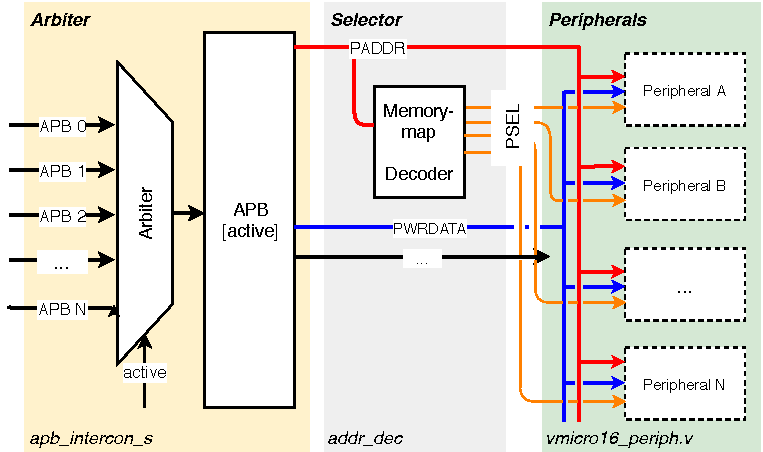
\includegraphics[width=0.8\textwidth]{decoder}
\caption{Schematic showing the address decoder (addr\_dec) accepting the active PADDR signal and outputting PSEL chip enable signals to each peripheral.}
\label{fig:decoder}
\end{figure}

\subsection{Decoder Optimisations}
Performing a 16-bit equality comparison of the \verb|PADDR| signal against each peripheral memory address consumes a significant amount of logic. Depending on the synthesis tools and FPGA features, a 16-bit comparator might require a fixed 16-bit value input to compare against (where the 0s are inverted) and a wide-AND to reduce and compare \cite{palchaudhuri2015high,salauyou2015designing}. An example 4-bit comparator is shown below in Figure \ref{fig:comparator}.

\begin{figure}[H]
\centering
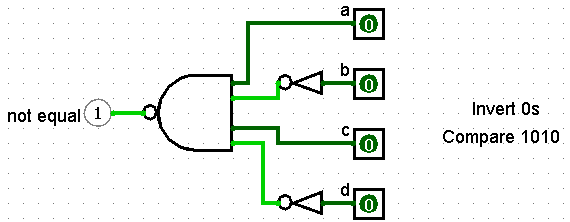
\includegraphics[width=0.5\textwidth]{comparator}
\caption{Example 4-bit binary comparator which compares the bits (a, b, c, d) to the constant value 1010. The 0s of the constant are inverted and then all are passed to a wide-AND.}
\label{fig:comparator}
\end{figure}

As we are targeting FPGAs, which use LUTs to implement combinatorial logic, we can conveniently utilise Verilog's \verb|==| operator on fairly large operands without worrying about consuming too many resources. The targeted FPGA devices in this project, the Cyclone V and Spartan 6, feature 6-input LUTs which allow 64 different configurations \cite{s6clb, cvclb}. Knowing this, we can design the address decoder to utilise the FPGA's LUTs more effectively and reduce it's footprint significantly.

We can use part of the \verb|PADDR| signal as a chip select and the other bits as sub-addresses to interface with the peripheral. The addressing bits are passed into the FPGA's 6-input LUTs which are programmed (via the bitstream) to output 1 or 0 depending on the address. Figure \ref{fig:comparatorlut} below shows a LUT based approach to address decoding which will utilise approximately 3 ALM modules (including error detection). This method of comparison (LUT based) is utilised in the \verb|addr_dec| module in \verb|apb_intercon.v|.

\begin{figure}[H]
\centering
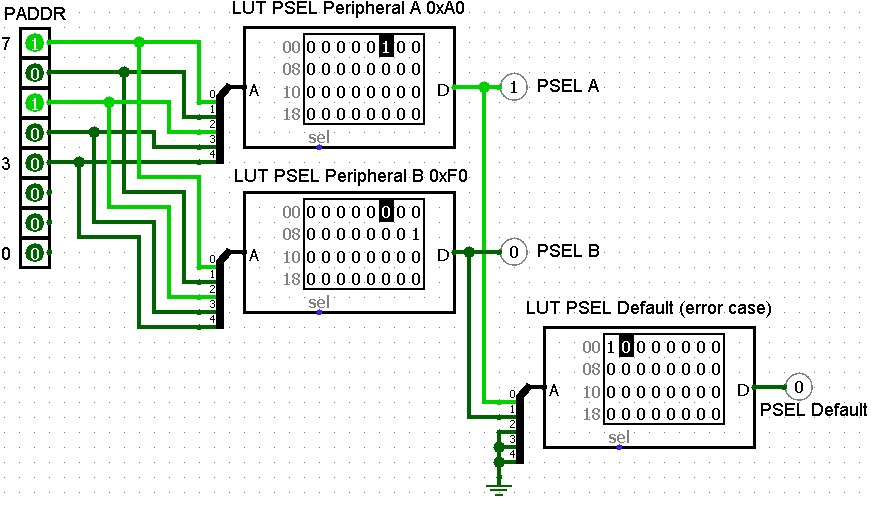
\includegraphics[width=0.8\textwidth]{comparatorlut}
\caption{Bits [7:3] of an 8-bit PADDR signal are used as inputs to 5-bit LUTs to generate a PSEL signal. In addition, a default error case is shown allowing the address decoder to detect incorrect PADDR values (e.g. if no PSEL signals are generated).}
\label{fig:comparatorlut}
\end{figure}

The address decoding methods discussed above are examples of \textit{full-address} decoding, where each bit (whether required or not) is compared. It is possible to further reduce the required logic by utilising \textit{partial-address} decoding \cite{tanenbaum2016structured}. Partial-address decoding can reduce logic requirements by not using all bits. For example, if bits in address \verb|0x0100| do not conflict with bits in other addresses (i.e. bit 8 is high in more than 1 address), then the address decoder needs only concern bit 8, not the other bits. This is visualised in Figure \ref{fig:partial} below. This method is utilised in the MMU's address decoder (module \verb|vmicro16_mmu| in \verb|vmicro16.v:181|). As this is an optimisation per core, significant resources can be saved when a large number of cores are used.

\begin{figure}[H]
\centering
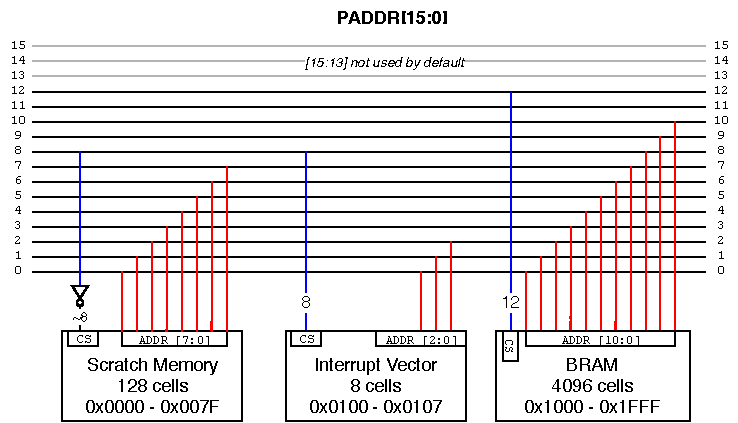
\includegraphics[width=0.8\textwidth]{partial}
\caption{Partial address decoding used by the Vmicro16 SoC design. Each peripheral shown only needs to decode a signal bit to determine if it is enabled.}
\label{fig:partial}
\end{figure}

\section{Memory Map}
The system-on-chip's memory map is shown below in Figure \ref{fig:memmap}. The addresses for each peripheral have been carefully chosen for both:
\begin{itemize}
\item Easy software access -- creating addresses via software requires few instructions (normally one to four \verb|MOVI| and \verb|LSHIFT| instructions to address \verb|0x0000| to  \verb|0xffff|), which increases software performance.
\item and Reducing address decoding logic -- most addresses can be decoded using partial decoding techniques.
\end{itemize}

\begin{figure}[H]
\centering
\begin{bytefield}{24}
	\memsection{1FFF}{1000}{8}{Shared Memory with Global Monitor \\ \vspace{.5cm} \tiny See vmicro16\_soc\_config.v}\\
	\bitbox[]{16}{} & \bitbox[]{16}{$\vdots$ \\[1ex]} \\
	
	\begin{rightwordgroup}{Shared peripherals}
	\memsection{0202}{0200}{3}{\nameref{sect:timer}}
	\end{rightwordgroup}\\
	\bitbox[]{16}{} & \bitbox[]{16}{$\vdots$ \\[1ex]} \\
	
	\begin{rightwordgroup}{Per-core instances}
	\memsection{0108}{}{1}{\nameref{sect:interrupts} Mask}\\
	\memsection{0107}{0100}{3}{\nameref{sect:interrupts} Vector}
	\end{rightwordgroup}\\
	
	\bitbox[]{16}{} & \bitbox[]{16}{$\vdots$ \\[1ex]} \\
	
	\begin{rightwordgroup}{Shared peripherals}
	\memsection{00B8}{}{1}{\nameref{sect:watchdog}}\\
	\memsection{00B7}{00B0}{3}{REGS0}\\
	\bitbox[]{16}{} & \bitbox[]{16}{$\vdots$ \\[1ex]} \\
	\memsection{00A1}{00A0}{2}{UART0}\\
	\bitbox[]{16}{} & \bitbox[]{16}{$\vdots$ \\[1ex]} \\
	\memsection{0092}{}{1}{GPIO2}\\
	\memsection{0091}{}{1}{GPIO1}\\
	\memsection{0090}{}{1}{GPIO0}
	\end{rightwordgroup}\\
	\bitbox[]{16}{} & \bitbox[]{16}{$\vdots$ \\[1ex]} \\
	
	\begin{rightwordgroup}{Per-core instances}
	\memsection{008F}{0080}{3}{16 Special Registers}\\
	\memsection{007F}{0000}{8}{Scratch Memory \\ \vspace{.5cm} \tiny See vmicro16\_soc\_config.v}
	\end{rightwordgroup}\\
	
\end{bytefield}
\caption{Memory map showing addresses of various memory sections.}
\label{fig:memmap}
\end{figure}

\chapter{Interrupts}
\label{sect:interrupts}
{%\hypersetup{linkcolor=black}
\startcontents[chapters]
\printcontents[chapters]{}{1}{}
}
\noindent\\
This section describes the design, considerations, and implementation, of interrupt functionality within the Vmicro16 processor.

\section{Why Interrupts?}
Interrupts are used to enable asynchronous behaviour within a processor.

Interrupts are commonly used to signal actions from asynchronous sources, for example an input button or from a UART receiver signalling that data has been received.

\section{Hardware Implementation}

\subsection{Context Switching}
When acting upon an incoming interrupt the current state the processor must be saved so that changes from the interrupt handler, such as register writes and branches, do not affect the current state. After the interrupt handler function signals it has finished (by using the \textit{Interrupt Return} \verb|intr| instruction) the saved state is restored.
In the case of the Vmicro16 processor, the program counter \verb|r_pc[15:0]| and register set \verb|regs| instance are the only states that are saved. Going forth, the terms \textit{normal mode} and \textit{interrupt mode} are used to describe what registers the processor should use when executing instructions.

When saving the state, to avoid clocking 128 bits (8 registers of 16 bits) into another register (which would increase timing delays and logic elements), a dedicated register set for the interrupt mode (\verb|regs_isr|) is multiplexed with the normal mode register set (\verb|regs|). Then depending on the mode (identified by the register \verb|regs_use_int|) the processor can easily switch between the two large states without significantly affecting timing.

The timing diagram in Figure \ref{fig:interrupts} visually describes this process.

\begin{figure}[h]
\centering
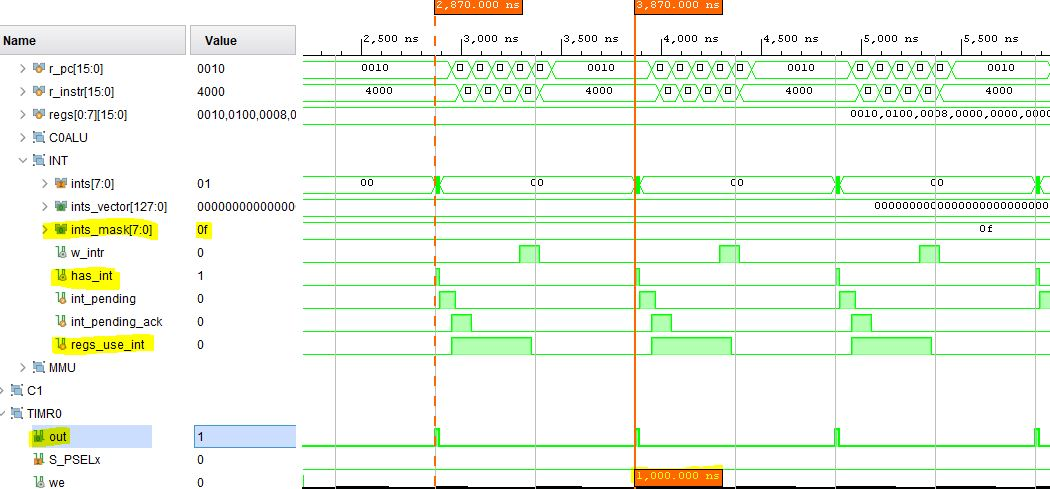
\includegraphics[width=\textwidth]{interrupts}
\caption{Time diagram showing the TIMR0 peripheral emitting a 1us periodic interrupt signal (out) to the processor. The processor acknowledges the interrupt (int\_pending\_ack) and enters the interrupt mode (regs\_use\_int) for a period of time. When the interrupt handler reaches the Interrupt Return instruction (indicated by w\_intr) the processor returns to normal mode and restores the normal state.}
\label{fig:interrupts}
\end{figure}

\section{Software Interface}
To enable software to 

\begin{figure}[H]
\centering
\begin{bytefield}[bitwidth=4ex, rightcurly=., rightcurlyspace=0pt]{16}
\bitheader[endianness=big]{0-15} \\
\begin{rightwordgroup}{0100 RW}
\bitbox{16}{Interrupt handler $0$}
\end{rightwordgroup} \\

\bitbox[]{16}{$\vdots$ \\[1ex]} \\
\begin{rightwordgroup}{0107 RW}
\bitbox{16}{Interrupt handler $7$}
\end{rightwordgroup} \\

\begin{rightwordgroup}{0108 RW}
\bitbox{8}{\color{lightgray}\rule{\width}{\height}} & \bitbox{8}{Interrupt bit mask}
\end{rightwordgroup}
\end{bytefield}
\caption{The interrupt vector consists of eight 16-bit values that point to memory addresses of the instruction memory to jump to.}
\label{fig:r_interrupts}
\end{figure}

\subsection{Interrupt Vector (0x0100-0x0107)}
The interrupt vector is a per-core register that is used to store the addresses of interrupt handlers. An interrupt handler is simply a software function residing in instruction memory that is branched to when a particular interrupt is received. 

\subsection{Interrupt Mask (0x0108)}
The interrupt mask is a per-core register that is used to mask/listen specific interrupt sources. This enables processing cores to individually select which interrupts they respond to. This allows for multi-processor designs where each core can be used for a particular interrupt source, improving the time response to the interrupt for time critical programs. The Interrupt Mask register is an 8-bit read/write register where each bit corresponds to a particular interrupt source and each bit corresponds with the interrupt handler in the interrupt vector.

\begin{figure}
\centering
\begin{bytefield}[bitwidth=4ex]{16}
& \bitlabel{8}{} &
& \bitlabel{6}{[7:2] User defined} &
& \bitlabel{1}{UART0 RX} 
& \bitlabel{1}{TIMR0} \\
\bitheader[endianness=big]{0-7,8,15} \\
  \bitbox{8}{\color{lightgray}\rule{\width}{\height}}
& \bitbox{1}{0}
& \bitbox{1}{0}
& \bitbox{1}{0}
& \bitbox{1}{0}
& \bitbox{1}{0}
& \bitbox{1}{0}
& \bitbox{1}{0}
& \bitbox{1}{0}
\end{bytefield}
\caption{Interrupt Mask register (0x0108). Each bit corresponds to an interrupt source. 1 signifies the interrupt is enabled for/visible to the core. Bits [7:2] are left to the designer to assign.}
\label{fig:r_interruptmask}
\end{figure}

\subsection{Software Example}
To better understand the usage of the described interrupt registers, a simple software program is described below. The following software program produces a simple and power efficient routine to initialise the interrupt vector and interrupt mask.

% pip install pygments-arm
\begin{minted}[fontsize=\footnotesize,linenos,,baselinestretch=0.8]{arm}
entry:
    // Set interrupt vector at 0x100
    // Move address of isr0 function to vector[0]
    movi    r0, isr0
    // create 0x100 value by left shifting 1 8 bits
    movi    r1, #0x1
    movi    r2, #0x8
    lshft   r1, r2
    // write isr0 address to vector[0]
    sw      r0, r1
    
    // enable all interrupts by writing 0x0f to 0x108
    movi    r0, #0x0f
    sw      r0, r1 + #0x8
    halt                  // enter low power idle state
    
isr0:                     // arbitrary name
    movi    r0, #0xff     // do something
    intr                  // return from interrupt
\end{minted}

A more complex example software program utilising interrupts and the TIMR0 interrupt is described in section \ref{sect:timr0_code}.

\section{Design Improvements}
The hardware and software interrupt design have changed throughout the projects cycle. In initial versions of the interrupt implementation, the software program, while waiting for an interrupt, would be in a tight infinite loop (branching to the same instruction). This resulted in the processor using all pipeline stages during this time. The pipeline stages produce many logic transitions and memory fetches which raise power consumption and temperatures. This is quite noticeable especially when running on the Spartan-6 LX9 FPGA.

To improve this, it was decided to implement a new state within the processor's state machine that, when entered, did not produce high frequency logic transitions or memory fetches. The \verb|HALT| instruction was modified to enter this state and the only way to leave is from an interrupt or top-level reset. This removes the need for a software infinite loop that produces high frequency logic transitions (decoding, ALU, register reads, etc.) and memory fetches.

\newpage
\chapter{Peripherals}
{%\hypersetup{linkcolor=black}
\startcontents[chapters]
\printcontents[chapters]{}{1}{}
}
\noindent\\
To provide user's with useful functionality, common system-on-chip peripherals were created. This section describes each peripheral and it's design decisions.

\section{Special Registers}
From the software perspective, it is important for both the developer and software algorithms to know the target system's architecture to better utilise
the resources available to them.
Software written for one architecture with $N$ cores must also run on an architecture with $M$ cores. To enable such portability, the software must query the system for information such as: number of processor cores and the current core identifier. Without this information, the developer would be required to produce software for each individual architecture (e.g. an Intel i5 with 4 cores or an Intel i7 with 8 cores, or an NVIDIA GTX 970 with.


\section{Watchdog Timer}
\label{sect:watchdog}
In any multi-threaded system there exists the possibility for a deadlock -- a state where all threads are in a waiting state -- and algorithm execution is forever blocked. This can occur either by poor software programming or incorrect thread arbitration by the processor. A common method of detecting a deadlock is to make each thread signal that it is not blocked by resetting a countdown timer. If the countdown timer is not reset, it will eventually reach zero and it is assumed that all threads are blocked as none have reset the countdown.

In this system-on-chip design, software can reset the watchdog timer by writing any 16-bit value to the address \verb|0x00B8|.

This peripheral is optional and can be enabled using the configuration parameters described in \nameref{sect:config}.

\begin{figure}[H]
\centering
\begin{bytefield}[bitwidth=4ex, rightcurly=., rightcurlyspace=0pt]{16}
\bitheader[endianness=big]{0-15} \\
\begin{rightwordgroup}{00B8 W}
\bitbox{16}{Reset Watchdog}
\end{rightwordgroup}
\end{bytefield}
\end{figure}

\section{GPIO Interface}
\begin{figure}[H]
\centering
\begin{bytefield}[bitwidth=4ex, rightcurly=., rightcurlyspace=0pt]{16}
\bitheader[endianness=big]{0-15} \\
\begin{rightwordgroup}{0090 RW}
\bitbox{16}{GPIO0 Output}
\end{rightwordgroup} \\
\begin{rightwordgroup}{0091 RW}
\bitbox{16}{GPIO1 Output}
\end{rightwordgroup} \\
\begin{rightwordgroup}{0092 R}
\bitbox{16}{GPIO1 Input}
\end{rightwordgroup}
\end{bytefield}
\end{figure}


\section{Timer with Interrupt}
\label{sect:timer}
\begin{figure}[H]
\centering
\begin{bytefield}[bitwidth=4ex, rightcurly=., rightcurlyspace=0pt]{16}
\bitheader[endianness=big]{0-15} \\
\begin{rightwordgroup}{0200 RW}
\bitbox{16}{Load Value}
\end{rightwordgroup} \\
\begin{rightwordgroup}{0201 W}
\bitbox{13}{\color{lightgray}\rule{\width}{\height}} &
\bitbox{1}{I} &
\bitbox{1}{R} &
\bitbox{1}{S}
\end{rightwordgroup} \\
\begin{rightwordgroup}{0202 W}
\bitbox{16}{Prescaler}
\end{rightwordgroup}
\end{bytefield}
\end{figure}


\section{UART Interface}
\begin{figure}[H]
\centering
\begin{bytefield}[bitwidth=4ex, rightcurly=., rightcurlyspace=0pt]{16}
\bitheader[endianness=big]{0,1,7,8,15} \\
\begin{rightwordgroup}{00A0 W}
\bitbox{8}{\color{lightgray}\rule{\width}{\height}} & \bitbox{8}{Transmit Data}
\end{rightwordgroup} \\
\begin{rightwordgroup}{00A1 R}
\bitbox{8}{\color{lightgray}\rule{\width}{\height}} & \bitbox{8}{Receive Data}
\end{rightwordgroup} \\
\begin{rightwordgroup}{00A2 R/W}
\bitbox{14}{\color{lightgray}\rule{\width}{\height}} & \bitbox{1}{E} & \bitbox{1}{I}
\end{rightwordgroup}
\end{bytefield}
\end{figure}



\chapter{Multi-core Communication}
\startcontents[chapters]
\printcontents[chapters]{}{1}{}

\noindent\\
So far we have discussed the features and design of the Vmicro16 system-on-chip. This section will discuss the multi-processing functionality and how to use it.

\section{Introduction}
Multi-processing functionality is the primary deliverable of this project.

\subsection{Design Goals}
\begin{itemize}
\item \textbf{Support common synchronisation primitives.}\\
Software should be able to implement common synchronisation primitives, such as mutexes, semaphores, and memory barriers, to perform atomic operations and avoid race conditions, which are critical in parallel and concurrent software applications.

\item \textbf{Context identification.}\\
The SoC should expose configuration information such as: the number of processing cores, amount of shared and scratch memory, and the \verb|CORE_ID|, to each thread.

\end{itemize}


\begin{figure}[h]
\centering
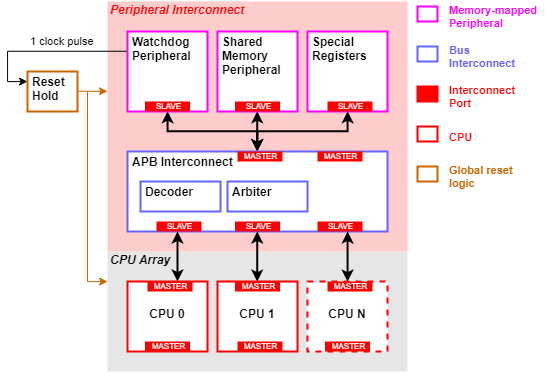
\includegraphics[width=0.7\textwidth]{multicore}
\caption{Block digram showing the main multi-processing components: the CPU array and a peripheral interconnect used for core synchronisation.}
\label{fig:multicore}
\end{figure}

\subsection{Context Identification}
A goal of the multi-processing functionality of this project is allow software written for it to be run on any number of cores. This means that a software program will scale to use all cores in the SoC without needing to rewrite the software. To enable this functionality, the software must be able to read contextual information about the SoC, such as the number of cores, how much global and scratch memory is available, and what the \verb|CORE_ID| of the current core is. 

This information is provided through the Special Registers peripheral (0x0080 - 0x008F), shown in \cref{fig:multicore}. This register set provides relevant information for writing software that can dynamically scale for various SoC configurations.

\begin{figure}[H]
\centering
\begin{bytefield}[bitwidth=4ex, rightcurly=., rightcurlyspace=0pt]{16}
\bitheader[endianness=big]{0-15} \\
\begin{rightwordgroup}{0080 R}
\bitbox{8}{\color{lightgray}\rule{\width}{\height}} & \bitbox{8}{CORE\_ID}
\end{rightwordgroup} \\
\begin{rightwordgroup}{0081 R}
\bitbox{8}{\color{lightgray}\rule{\width}{\height}} & \bitbox{8}{NUM\_CORES}
\end{rightwordgroup} \\
\begin{rightwordgroup}{0082 R}
\bitbox{16}{SHARED\_MEMORY cells \tiny(default 4096)}
\end{rightwordgroup} \\
\begin{rightwordgroup}{0083 R}
\bitbox{8}{\color{lightgray}\rule{\width}{\height}} & \bitbox{8}{NUM\_PERIPHERALS}
\end{rightwordgroup} \\
\begin{rightwordgroup}{0084 RW}
\bitbox{16}{SCRATCH\_MEMORY cells \tiny(default 64)}
\end{rightwordgroup} \\
\begin{rightwordgroup}{0085 RW}
\bitbox{16}{User defined}
\end{rightwordgroup} \\
\bitbox[]{16}{$\vdots$ \\[1ex]} \\
\begin{rightwordgroup}{008F RW}
\bitbox{16}{User defined}
\end{rightwordgroup}
\end{bytefield}
\caption{Vmicro16 Special Registers layout (0x0080 - 0x008F).}
\end{figure}

\subsection{Thread Synchronisation}
In multi-threaded software it is important 

The mutex functionality is implemented using a similar scheme to that of ARM's \textit{Global Monitor} \cite{armgmonitor}.

\subsubsection{Mutexes}
In software, a mutex is an object used to control access to a shared resource. The term \textit{object} is used as it's implementation is normally platform dependant, meaning that the processor may provide a hardware mechanism or is left for the operating system to provide.

In this project, mutexes are provided by the processor through the Shared Memory Peripheral (0x1000 to 0x1FFF) which provides a large RAM-style memory accessible by all cores through the peripheral interconnect bus. This large memory is explicitly defined to use the FPGA's BRAM blocks using Xilinx's Verilog \verb|ram_style="block"| attribute to avoid wasting LUTs when using high core counts. The peripheral allows each memory cell to be \textit{locked}, meaning that only the cell owner can modify it's contents. This is implemented by using another large memory, \verb|locks|, to store the $\verb|CORE_ID| + 1$ of the owner, as shown in \cref{fig:lock}. In this system, a lock containing the value 0 indicates an unlocked cell. As \verb|CORE_ID|s are indexed from zero, 1 is arithmetically added to each cell. For example, if core \#2 wants to lock a memory cell, the value 3 is written to the lock.

\begin{listing}[h]
\centering
\begin{minted}{verilog}
reg [15:0]           ram   [0:8191]; // 16KB large RAM memory
reg [clog2(CORES):0] locks [0:8181]; // memory cell owner
\end{minted}
\caption{RAM and lock memories instantiated by the shared memory peripheral.}
\label{fig:lock}
\end{listing}

To lock and unlock cells, the instructions \verb|LWEX| and \verb|SWEX| instructions are used. These instructions are similar to the \verb|LW/SW| instructions but provide locking functionality. The \textit{EX} in the instruction names indicate \textit{exclusive access}. \verb|LWEX| is used to read memory contents  (like \verb|LW|) and also lock the cell if not already locked. If a core attempts to lock an already locked cell, the lock does not change. Unlocking is done by the \verb|SWEX| instruction, which conditionally writes to the memory cell if it is locked by the same core. Unlike \verb|SW|, \verb|SWEX| returns a zero for success and one for failure if it is locked by another core.

\begin{wrapfigure}{L}{0.5\textwidth}
\centering
\begin{minted}[fontsize=\footnotesize,
    baselinestretch=0.8,]{arm}
lock_mutex:
	// attempt lock
	lwex r0, r1
	// check success
	swex r0, r1
	cmp  r0, r3
	// if not equal (NE), retry
	movi r4, lock_mutex
	br   r4, BR_NE
critical:
    // core has the mutex
\end{minted}
\caption{Assembly code for locking a mutex. r1 is the address to lock. r3 is zero. r4 is the branch address.}
\label{fig:codemutex}
\end{wrapfigure}

\cref{fig:codemutex} shows a simple assembly function to lock a memory cell.

\if 0
\begin{figure}[h]
\centering
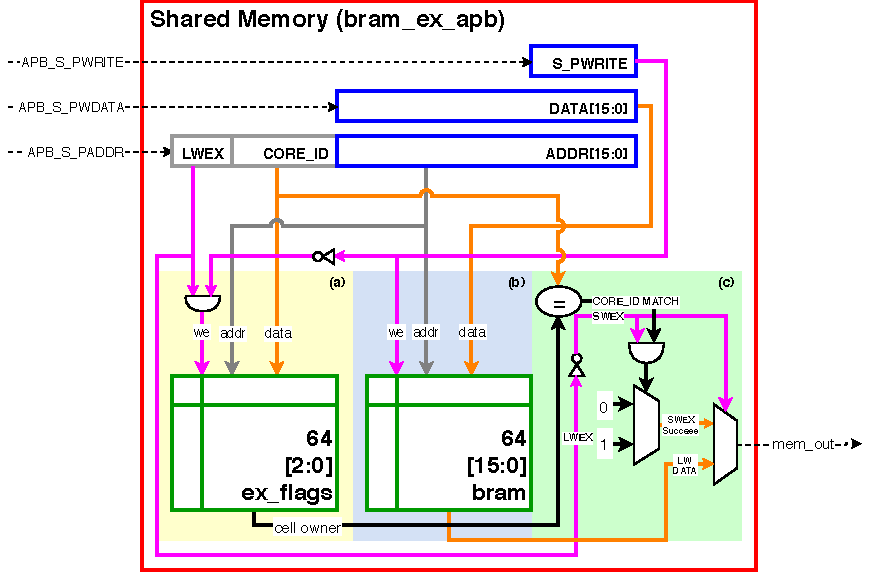
\includegraphics[width=\textwidth]{bram_ex}
\caption{Shared Memory Peripheral schematic showing RAM memory and lock memories.}
\label{fig:bram_ex}
\end{figure}
\fi


\subsubsection{Barriers}
Barriers are a useful software sequence used to block execution until all other threads (or a subset) have reached the same point. Barriers are often used for broadcast and gather actions (sending values to each core or receiving them). They are also used to synchronise program execution if some threads have more work to do than others.

\begin{wrapfigure}{L}{0.5\textwidth}
\centering
\begin{minted}[fontsize=\footnotesize,
    baselinestretch=0.8,]{arm}
barrier_reached:
    // load latest count
    lwex    r0, r5
    // try increment count
    // increment by 1
    addi    r0, r3 + #0x01
    // attempt store
    swex    r0, r5

    // check success (== 0)
    cmp     r0, r3
    // branch if failed
    movi    r4, barrier_reached
    br      r4, BR_NE

barrier_wait:
    // load the count
    lw      r0, r5
    // compare with number of threads
    cmp     r0, r7
    // jump back to barrier if not equal
    movi    r4, barrier_wait
    br      r4, BR_NE
\end{minted}
\caption{Assembly code for a memory barrier. Threads will wait in the barrier\_wait function until all other threads have reached that code point.}
\label{fig:codebarrier}
\end{wrapfigure}

The Vmicro16 processor provides barrier synchronisation through the Shared Memory Peripheral. Like the mutex code, the barrier code uses the \verb|LWEX| and \verb|SWEX| instructions to lock a memory cell. Instead of immediately checking the lock as an abstract object, the barrier code treats the cell as a normal memory cell containing a numeric value. \cref{fig:codebarrier} shows a software example of this. When the \verb|barrier_reached| code is reached, the code will increment the shared memory value by 1, indicating that the number of threads that have reached this point has increased by one (r5). The \verb|barrier_wait| function is then entered which waits until this numeric value (r5) is equal to the number of threads (r7) in the system. If this is true, then all threads have reached the \verb|barrier_wait| function and can continue with normal program execution.

\section{Design Challenges}
\subsection{Memory Constraints}


\begin{figure}[H]
\centering
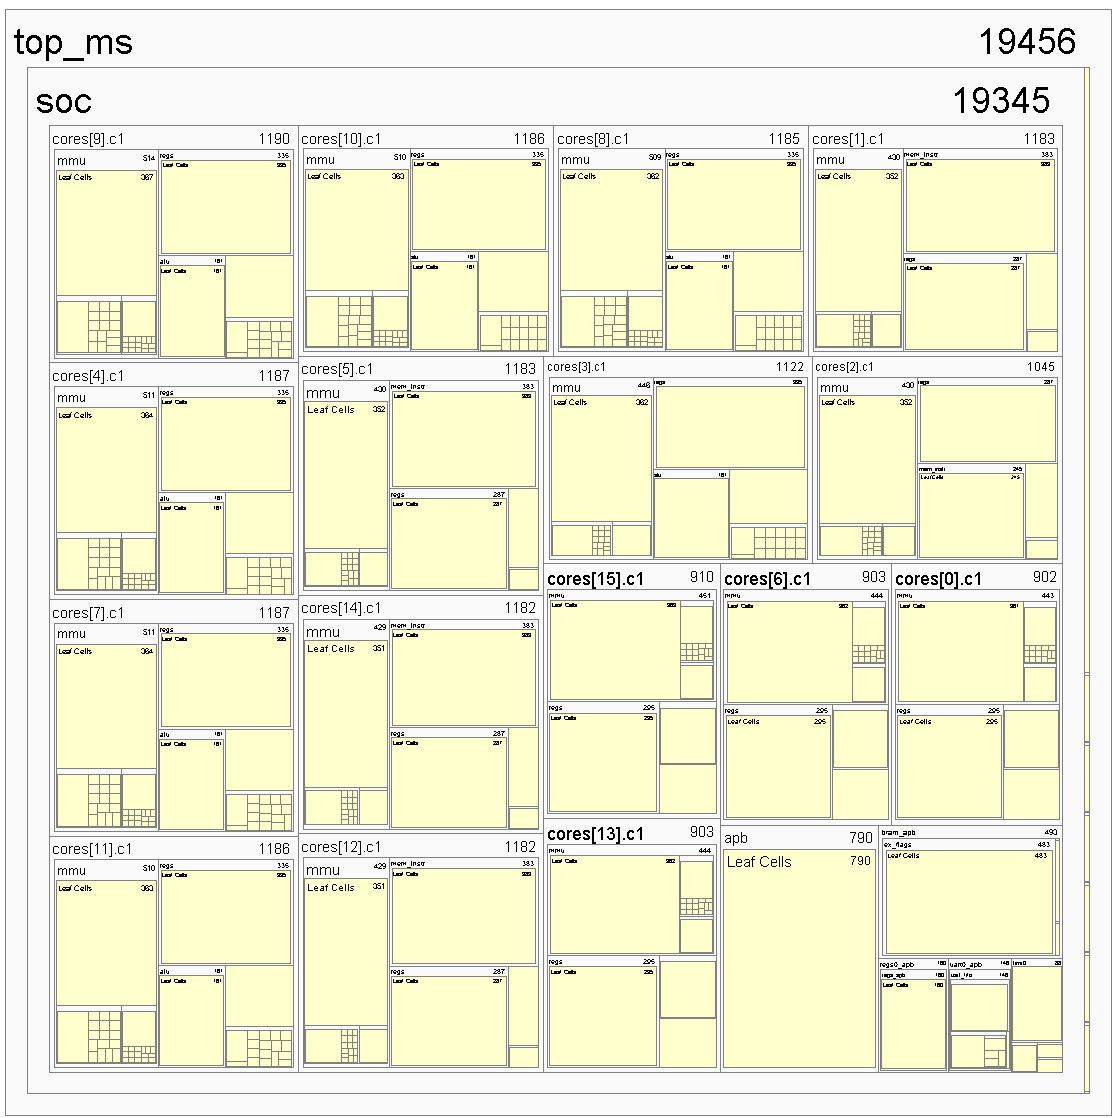
\includegraphics[width=13cm]{soc_layout_schem}
\caption{•}
\label{}
\end{figure}
\chapter{Analysis \& Results}
\startcontents[chapters]
\printcontents[chapters]{}{1}{}
\noindent\\
So far the system's design, implementation, and example usage, has been presented and discussed.

\section{Introduction}
This chapter presents analytic information

\section{Implementation Analysis}
This section analysis the synthesised and implemented system-on-chip design to see the effect of increasing core counts.

\subsection{Design Size}
\subsubsection{Implementation}
On a minimal system-on-chip configuration, with one core and minimal peripherals and features (no reprogramming, no interrupts, no UART), the design requires as few as 700 LUTs with the processor core requiring approximately 300-400 LUTs.

\subsubsection{Memory Constraints}
As discussed in \cref{sec:singlecore} \nameref{sec:singlecore}, each processor core features two memories: instruction and scratch memory, which can both map onto synchronous, single-port, FPGA BRAM blocks. While this will reduce LUT requirements in designs with few cores, it becomes a non-trivial problem as the core counts increase. FPGAs have a fixed number of hard-BRAM blocks available for inference by the HDL compiler, for example the low-end Xilinx Spartan-6 XC6SLX9 FGPA features 32 18 Kb BRAM blocks \cite[p.~2]{s6fam}, and the Cyclone V 5CSEMA5F31C6N (used in the DE1-SoC) has 397 10 Kb blocks \cite[p.~22]{cvfam}.

\begin{figure}[h]
\begin{subfigure}{.5\textwidth}
  \centering
  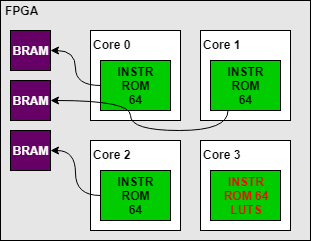
\includegraphics[width=.7\linewidth]{bram_limit}
  \caption{A theoretical FPGA device with 3 BRAM blocks running a 4-core design. Each core can map onto a BRAM block, however as there are more cores than BRAM blocks available, some core memories will be implemented as distributed RAM, or in the worse case using ALMs.}
  \label{fig:bram_limita}
\end{subfigure}%
\begin{subfigure}{.5\textwidth}
  \centering
  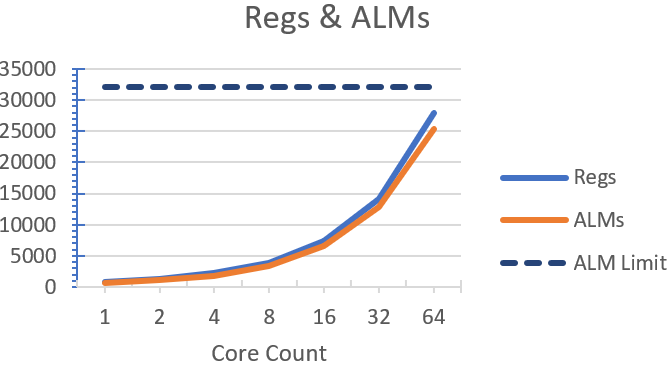
\includegraphics[width=1.2\linewidth]{sizes_regs}
  \caption{DE1-SoC (Cyclone V) resource utilisation with various core counts.}
  \label{fig:bram_limitb}
\end{subfigure}
\caption{}
\label{fig:bram_limit}
\end{figure}

As shown in \cref{fig:bram_limita}, as the number of processor cores increases, they eventually outnumber the available BRAM blocks resulting in their memories being implemented in either distributed RAMs or ALMs, both of which can consume significant logic resources of the FPGA which reduces the maximum possible core count.

Figure \cref{fig:bram_limitb} shows the FPGA resource requirements for the DE1-SoC board featuring the Cyclone V FPGA. Approximately 32 cores can be instantiated before the all the available registers and ALMs are consumed.

\subsubsection{Reducing Memory Requirements}
\label{sec:anal_memory}
As shown in \cref{fig:bram_limita}, each core has it's own instruction read-only memory. These memories have identical contents which presents an opportunity for optimisation. In the proposed design in \cref{fig:bram_limit_sola}, this memory is removed from each core and is instead available through a dedicated shared bus. This approach can be configured to be used in the Vmicro16 SoC through the \verb|DEF_CORE_HAS_INSTR_MEM| parameter in \verb|vmicro16_soc_config.v|, which enables the \textit{Instruction Memory Interconnect} shown in \cref{fig:watchdog}.

As shown in \cref{fig:bram_limit_solb}, the resource requirements using this shared memory approach is significantly less than having an instruction memory per-core. On the DE1-SoC, 64 cores can now be instantiated with a few thousand regs and ALMs left for other logic.


\begin{figure}[H]
\begin{subfigure}{.5\textwidth}
  \centering
  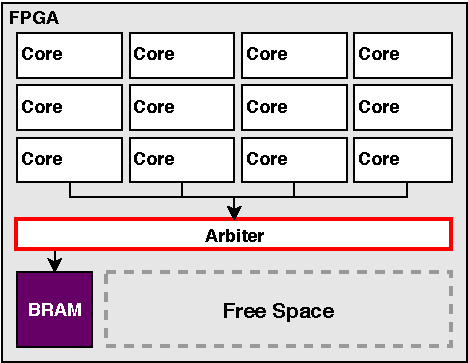
\includegraphics[width=.7\linewidth]{bram_limit_sol}
  \caption{A multi-core architecture where each core must fetch instructions externally from a global memory.}
  \label{fig:bram_limit_sola}
\end{subfigure}%
\begin{subfigure}{.5\textwidth}
  \centering
  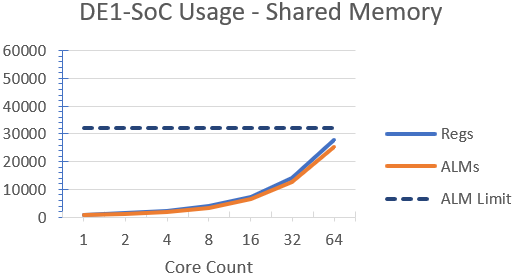
\includegraphics[width=1.2\linewidth]{sizes_regs_shared}
  \caption{DE1-SoC (Cyclone V) resource utilisation with various core counts using shared instruction memory.}
  \label{fig:bram_limit_solb}
\end{subfigure}
\caption{}
\label{fig:bram_limit_sol}
\end{figure}

Whilst this is a significant resource saving opportunity, it does have significant drawbacks. In the shared instruction memory approach, each core must now fetch it's instruction from the instruction memory interconnect which is subject to the arbiter and it's scheduling algorithm. The arbiter uses the same algorithm as the peripheral interconnect arbiter meaning that cores receive access incrementally, and as discussed in \cref{sec:multimaster}, this results in significant delays in many-core designs. This drawback is further explained in \cref{sec:result_results}.



\subsection{Maximum Frequency}
\begin{figure}[h]
\centering
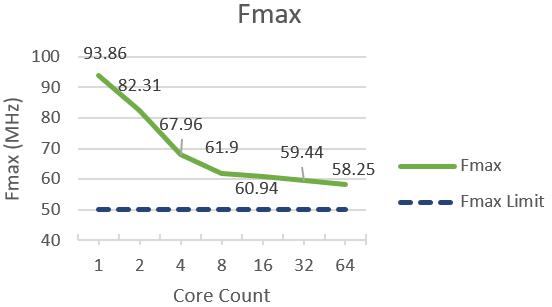
\includegraphics[width=0.6\textwidth]{sizes_fmax}
\caption{Cyclone V maximum design frequency for various core count configurations.}
\label{fig:sizes_fmax}
\end{figure}

\section{Scenario Performance}
To evaluate the performance of the system-on-chip, scenarios encompassing computational problems that are reflective of real-world applications are compiled and ran on the design.

\subsection{Scenario Overview}
\label{sec:scenario}
The scenario is a software program that runs a parallel implementation of the summation function, i.e. \verb|sum [1..10]| which returns 55. While this may seem too simple at first to measure performance of a multi-core system-on-chip, the function is actually quite appropriate as it encompasses various parallel problems, such as: a fixed time/size serial part; broadcasting of the data set (in this case the range of the summation); thread synchronisation (to know when the data is ready and to schedule gathering of intermediary results); and is highly scalable.
\\\\
The summation task flow is as follows:
\begin{enumerate}
\item Root (core \#0) broadcasts the range of the summation (i.e. sum 1 to 10) to all cores via the global shared memory.
\item Non-root cores wait for this broadcast to finish (memory barrier), then calculate their own subset of the range to sum. For example, if Root broadcasts that there are 240 samples and 10 cores in the system, each core calculates the subset size:

\begin{equation}
240/10 = 24
\end{equation} calculations starting from:
\begin{equation}
{ID_{CORE}} * 24
\end{equation}
For example, Core \#5 will start its 24 sample subset summation from
\begin{equation}
5 * 24 = 120
\end{equation}
effectively performing \verb|sum [120..123]|.

\item All cores perform an intermediary summation over their subset of the range (serial part).
\item All cores attempt to add their intermediary result to a global sum value in global shared memory (mutex).
\item All cores halt, signalling that their work has been committed to the global shared memory and have finished the program.
\end{enumerate}

This program is written in assembly in the file \verb|sw/demos/asm/sum64.s| and can be compiled using the assembly compiler (developed for deliverable \ref{ed:compiler}) using the command below. The assembly compiler outputs the file \verb|asm.s.hex| containing hex instruction words for use in Verilog's \verb|$readmemh| function. This data is used for each core's instruction memory. The assembly program is also shown in \cref{sec:64coresum}.
\\
\mintinline{bash}{                      python sw/asm.py sw/demos/asm/sum64.s}

\subsection{Performance Measurements}
Behavioural simulation is used to measure the following metrics to estimate general performance of the system-on-chip:
\begin{itemize}
\item Total program run-time.\\This is the time from when the reset signal is de-asserted to when all cores have halted. Each core has an output \verb|halt| signal which the SoC can use to determine if all cores have halted using \verb|wire all_halted = &core_halts;|. 

\item Time spent on the serial part.\\The serial part of this scenario consists of the intermediary summation of it's subset range. As each core is performing this task, the average will be used.

\item Time spent on communication.\\This includes time spent on thread synchronisation, i.e. waiting for the global memory to become available and waiting on the root to finish broadcast. Again, the average time will be used.

\item Time spent fetching instructions.\\Instruction fetches occur during stage \verb|STAGE_IF| of the pipeline. The behavioural test bench will record the number of clock cycles each core spends in this state, then calculate the average time spent fetching instructions. 
\end{itemize}

These measurements are recorded using non-synthesisable Verilog code in both the testbench and module code (\verb|vmicro16_soc.v|).

\subsection{Performance Results}
\label{sec:result_results}
The scenario program was simulated on system configuration with 1 to 30 cores with a 50 MHz clock.
\cref{fig:alg_time} shows the time breakdown of the multi-core system-on-chip running the scenario problem with various core counts. In these measurements all cores feature a small instruction memory which is accessed in constant time (one clock), and so this fetch time is not shown in the chart. 

\begin{figure}[h]
\centering
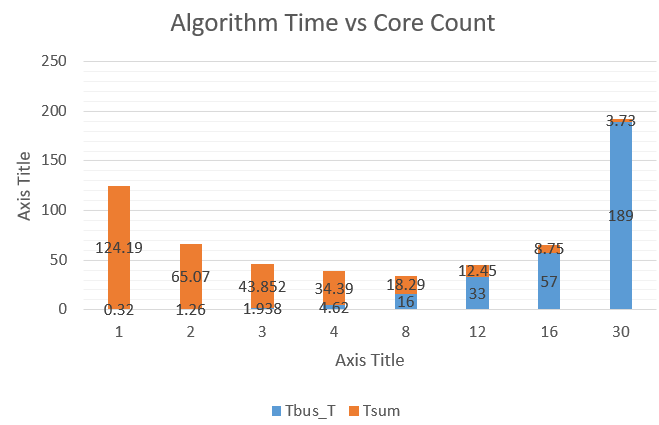
\includegraphics[width=0.7\textwidth]{alg_time}
\caption{Chart showing how the communication times (Tbus) and serial times (Tsum) changes with core count.}
\label{fig:alg_time}
\end{figure}

The chart shows the expected shape for software parallel performance -- as the number of cores increase, each core's problem space is reduced resulting in faster completion of the summation part, and an increasing amount of time is spent on thread communication. This result matches my CUDA and MPI parallelism performance analysis results conducted in 2018 \cite{soft354}.

It can be seen that the total run-time is fastest near 8 cores and increases at this point when using more cores. This is likely due to the small summation range per core -- with 30 cores just 8 samples per core are summed, which is extremely overkill and not representative of what a 30-core plus system should be used for.

If a much larger summation range was used (effectively representing a more appropriate scenario for systems with high core counts), the chart shape would stretch horizontally, resulting in the fastest time being on a higher core count than 8.

With high-core counts (16+) it can be seen that the communication time (Tbus\_T) increases significantly. This is likely due to the rotating arbiter design. As discussed in \cref{sec:multimaster}, the arbiter grants bus access to the next core incrementally after the previous core finishes. For large core systems, this can result in large time penalties. For example, if core \#30 is blocking all other cores and the arbiter is lagging behind granting access to core \#5, it will take a significant amount of time for the arbiter to reach core 30 to unblock the system.

\subsection{Memory}
As previous discussed in \cref{sec:

\begin{figure}[h]
\centering
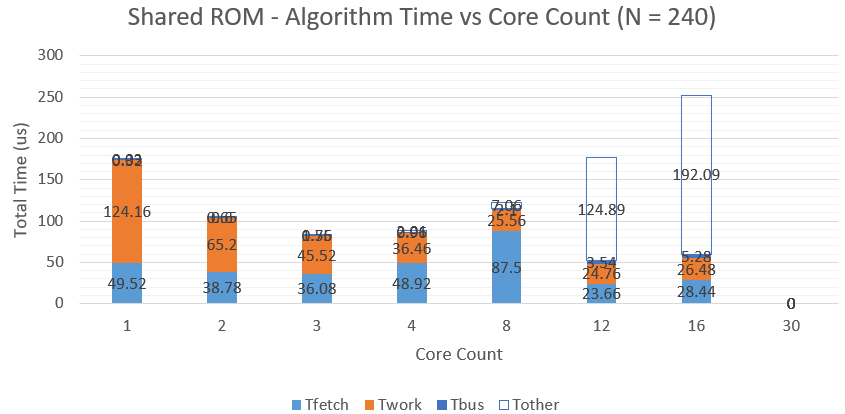
\includegraphics[width=0.7\textwidth]{alg_time_shared}
\caption{Similar to \cref{fig:alg_time} but using shared instruction memory to reduce block memory requirements per core.}
\label{fig:alg_time_shared}
\end{figure}


\section{Analysis Review}
There are several takeaways from these results:
\begin{enumerate}
\item Use an appropriate number of cores for the dataset size.\\Too few cores result in longer work times and shorter communication times, and too many cores results in shorter work times and longer communication times.

\item Use an appropriate arbitration scheme to prevent blocking the system for too long.\\
In this design, and likely others, the blocking core is known by the global shared memory (via the locking cells) meaning that this information can be passed to the arbiter to give priority, while still avoiding deadlocks, to the blocking core.

\item Use an appropriate number of cores and still have space for other business logic.

\item More cores may result in lower clock frequencies.\\From \cref{fig:sizes_fmax}, the single-core design can be ran at $\approx$95 MHz while the 4-core design only $\approx$65 MHz (a $\approx$30\% decrease). The parallel speed improvements from having more cores may be less than a single fast core.
\end{enumerate}

System designers should experiment with their algorithm and these takeaways to determine the approximate number of processor cores for their requirements, be that algorithm time, size, clock frequency, or compilation time.



\chapter{Conclusion}
\section{Future Work}
\section{Conclusion}
















\include{chapter_improv}

%TC:ignore
\clearpage
\bibliography{refs}
\addcontentsline{toc}{chapter}{References}
\begin{appendices}
\startcontents[chapters]

\chapter{Configuration Options}
\label{sect:config}
\startcontents[chapters]
\printcontents[chapters]{}{1}{}

\noindent\\
The following configuration options are defined in \verb|vmicro16_soc_config.v|.

\section{SoC Options}
\begin{table}[H]
\centering
\label{tab:isa}
\begin{tabularx}{\textwidth}{l|l|p{8cm}}
Macro      & Default & Purpose                         \\ 
\hline
CORES  & 4       & Number of CPU cores in the SoC  \\
SLAVES & 7       & Number of peripherals  \\    
DEF\_USE\_WATCHDOG &  & Enable watchdog module to detect deadlocks and infinite loops \\    
\end{tabularx}
\caption{SoC Configuration Options}
\end{table}

\section{Core Options}
\begin{table}[H]
\centering
\begin{tabular}{l|l|p{8cm}}
Macro                      & Default & Purpose                                     \\ 
\hline
DATA\_WIDTH                & 16      & Width of CPU registers in bits              \\
DEF\_CORE\_HAS\_INSTR\_MEM & //      & Enable a per core instruction memory cache  \\
DEF\_MEM\_INSTR\_DEPTH     & 64      & Instruction memory cache per core           \\
DEF\_MEM\_SCRATCH\_DEPTH   & 64      & RW RAM per core                             \\
DEF\_ALU\_HW\_MULT        & 1       & Enable/disable HW multiply (1 clock)        \\
FIX\_T3                    & //      & Enable a T3 state for the APB transaction \\

DEF\_GLOBAL\_RESET           & //      & Enable synchronous reset logic \\

DEF\_USE\_REPROG           & //      & Programme instruction memory via UART0. Requires DEF\_GLOBAL\_RESET\\
\end{tabular}
\caption{Core Options}
\label{tab:isa}
\end{table}

\section{Peripheral Options}
\begin{table}[H]
\centering
\begin{tabular}{l|l|l}
Macro              & Default  & Purpose                                              \\ 
\hline
APB\_WIDTH         &          & AMBA APB PADDR signal width                          \\
APB\_PSELX\_GPIO0  & 0        & GPIO0 index                                          \\
APB\_PSELX\_UART0  & 1        & UART0 index                                          \\
APB\_PSELX\_REGS0  & 2        & REGS0 index                                          \\
APB\_PSELX\_BRAM0  & 3        & BRAM0 index                                          \\
APB\_PSELX\_GPIO1  & 4        & GPIO1 index                                          \\
APB\_PSELX\_GPIO2  & 5        & GPIO2 index                                          \\
APB\_PSELX\_TIMR0  & 6        & TIMR0 index                                          \\
APB\_BRAM0\_CELLS  & 4096     & Shared memory words                                  \\
DEF\_MMU\_TIM0\_S  & 16'h0000 & Per core scratch memory start/end address            \\
DEF\_MMU\_TIM0\_E  & 16'h007F & "                                                    \\
DEF\_MMU\_SREG\_S  & 16'h0080 & Per core special registers start/end address         \\
DEF\_MMU\_SREG\_E  & 16'h008F & "                                                    \\
DEF\_MMU\_GPIO0\_S & 16'h0090 & Shared GPIOn start/end address                       \\
DEF\_MMU\_GPIO0\_E & 16'h0090 & "                                                    \\
DEF\_MMU\_GPIO1\_S & 16'h0091 & "                                                    \\
DEF\_MMU\_GPIO1\_E & 16'h0091 & "                                                    \\
DEF\_MMU\_GPIO2\_S & 16'h0092 & "                                                    \\
DEF\_MMU\_GPIO2\_E & 16'h0092 & "                                                    \\
DEF\_MMU\_UART0\_S & 16'h00A0 & Shared UART start/end address                        \\
DEF\_MMU\_UART0\_E & 16'h00A1 & "                                                    \\
DEF\_MMU\_REGS0\_S & 16'h00B0 & Shared registers start/end address                   \\
DEF\_MMU\_REGS0\_E & 16'h00B7 & "                                                    \\
DEF\_MMU\_BRAM0\_S & 16'h1000 & Shared memory with global monitor start/end address  \\
DEF\_MMU\_BRAM0\_E & 16'h1FFF & "                                                    \\
DEF\_MMU\_TIMR0\_S & 16'h0200 & Shared timer peripheral start/end address            \\
DEF\_MMU\_TIMR0\_E & 16'h0202 & "                                                   
\end{tabular}
\caption{Peripheral Options}
\label{tab:isa}
\end{table}

\clearpage
\chapter{Code Listing}
\startcontents[chapters]
\printcontents[chapters]{}{1}{}

\section{vmicro16\_soc\_config.v}
Configuration file for configuring the vmicro16\_soc.v and vmicro16.v features.

\inputminted[
    linenos,
    fontsize=\scriptsize,
    baselinestretch=0.8,
]{verilog}{../../vmicro16/vmicro16_soc_config.v}

\section{top\_ms.v}
Top level module that connects the SoC design to hardware pins on the FPGA.
\inputminted[
    linenos,
    fontsize=\scriptsize,
    baselinestretch=0.8,
]{verilog}{../../vmicro16/top_ms.v}

\section{vmicro16\_soc.v}
\inputminted[
    linenos,
    fontsize=\scriptsize,
    baselinestretch=0.8,
]{verilog}{../../vmicro16/vmicro16_soc.v}


\section{vmicro16\_periph.v}
Various memory-mapped APB peripherals, such as GPIO, UART, timers, and memory.

\inputminted[
    linenos,
    fontsize=\scriptsize,
    baselinestretch=0.8,
]{verilog}{../../vmicro16/vmicro16_periph.v}

\section{vmicro16.v}
Vmicro16 CPU core module.

\inputminted[
    linenos,
    fontsize=\scriptsize,
    baselinestretch=0.8,
]{verilog}{../../vmicro16/vmicro16.v}


\end{appendices}
%TC:endignore


\end{document}


